% Generated by Sphinx.
\def\sphinxdocclass{report}
\documentclass[letterpaper,10pt,english]{sphinxmanual}
\usepackage[utf8]{inputenc}
\DeclareUnicodeCharacter{00A0}{\nobreakspace}
\usepackage{cmap}
\usepackage[T1]{fontenc}
\usepackage{babel}
\usepackage{times}
\usepackage[Bjarne]{fncychap}
\usepackage{longtable}
\usepackage{sphinx}
\usepackage{multirow}


\title{ownCloud User Manual}
\date{December 09, 2016}
\release{9.2}
\author{The ownCloud developers}
\newcommand{\sphinxlogo}{
\includegraphics{logo-blue.pdf}\par}
\renewcommand{\releasename}{Release}
\makeindex

\makeatletter
\def\PYG@reset{\let\PYG@it=\relax \let\PYG@bf=\relax%
    \let\PYG@ul=\relax \let\PYG@tc=\relax%
    \let\PYG@bc=\relax \let\PYG@ff=\relax}
\def\PYG@tok#1{\csname PYG@tok@#1\endcsname}
\def\PYG@toks#1+{\ifx\relax#1\empty\else%
    \PYG@tok{#1}\expandafter\PYG@toks\fi}
\def\PYG@do#1{\PYG@bc{\PYG@tc{\PYG@ul{%
    \PYG@it{\PYG@bf{\PYG@ff{#1}}}}}}}
\def\PYG#1#2{\PYG@reset\PYG@toks#1+\relax+\PYG@do{#2}}

\expandafter\def\csname PYG@tok@gd\endcsname{\def\PYG@tc##1{\textcolor[rgb]{0.63,0.00,0.00}{##1}}}
\expandafter\def\csname PYG@tok@gu\endcsname{\let\PYG@bf=\textbf\def\PYG@tc##1{\textcolor[rgb]{0.50,0.00,0.50}{##1}}}
\expandafter\def\csname PYG@tok@gt\endcsname{\def\PYG@tc##1{\textcolor[rgb]{0.00,0.27,0.87}{##1}}}
\expandafter\def\csname PYG@tok@gs\endcsname{\let\PYG@bf=\textbf}
\expandafter\def\csname PYG@tok@gr\endcsname{\def\PYG@tc##1{\textcolor[rgb]{1.00,0.00,0.00}{##1}}}
\expandafter\def\csname PYG@tok@cm\endcsname{\let\PYG@it=\textit\def\PYG@tc##1{\textcolor[rgb]{0.25,0.50,0.56}{##1}}}
\expandafter\def\csname PYG@tok@vg\endcsname{\def\PYG@tc##1{\textcolor[rgb]{0.73,0.38,0.84}{##1}}}
\expandafter\def\csname PYG@tok@m\endcsname{\def\PYG@tc##1{\textcolor[rgb]{0.13,0.50,0.31}{##1}}}
\expandafter\def\csname PYG@tok@mh\endcsname{\def\PYG@tc##1{\textcolor[rgb]{0.13,0.50,0.31}{##1}}}
\expandafter\def\csname PYG@tok@cs\endcsname{\def\PYG@tc##1{\textcolor[rgb]{0.25,0.50,0.56}{##1}}\def\PYG@bc##1{\setlength{\fboxsep}{0pt}\colorbox[rgb]{1.00,0.94,0.94}{\strut ##1}}}
\expandafter\def\csname PYG@tok@ge\endcsname{\let\PYG@it=\textit}
\expandafter\def\csname PYG@tok@vc\endcsname{\def\PYG@tc##1{\textcolor[rgb]{0.73,0.38,0.84}{##1}}}
\expandafter\def\csname PYG@tok@il\endcsname{\def\PYG@tc##1{\textcolor[rgb]{0.13,0.50,0.31}{##1}}}
\expandafter\def\csname PYG@tok@go\endcsname{\def\PYG@tc##1{\textcolor[rgb]{0.20,0.20,0.20}{##1}}}
\expandafter\def\csname PYG@tok@cp\endcsname{\def\PYG@tc##1{\textcolor[rgb]{0.00,0.44,0.13}{##1}}}
\expandafter\def\csname PYG@tok@gi\endcsname{\def\PYG@tc##1{\textcolor[rgb]{0.00,0.63,0.00}{##1}}}
\expandafter\def\csname PYG@tok@gh\endcsname{\let\PYG@bf=\textbf\def\PYG@tc##1{\textcolor[rgb]{0.00,0.00,0.50}{##1}}}
\expandafter\def\csname PYG@tok@ni\endcsname{\let\PYG@bf=\textbf\def\PYG@tc##1{\textcolor[rgb]{0.84,0.33,0.22}{##1}}}
\expandafter\def\csname PYG@tok@nl\endcsname{\let\PYG@bf=\textbf\def\PYG@tc##1{\textcolor[rgb]{0.00,0.13,0.44}{##1}}}
\expandafter\def\csname PYG@tok@nn\endcsname{\let\PYG@bf=\textbf\def\PYG@tc##1{\textcolor[rgb]{0.05,0.52,0.71}{##1}}}
\expandafter\def\csname PYG@tok@no\endcsname{\def\PYG@tc##1{\textcolor[rgb]{0.38,0.68,0.84}{##1}}}
\expandafter\def\csname PYG@tok@na\endcsname{\def\PYG@tc##1{\textcolor[rgb]{0.25,0.44,0.63}{##1}}}
\expandafter\def\csname PYG@tok@nb\endcsname{\def\PYG@tc##1{\textcolor[rgb]{0.00,0.44,0.13}{##1}}}
\expandafter\def\csname PYG@tok@nc\endcsname{\let\PYG@bf=\textbf\def\PYG@tc##1{\textcolor[rgb]{0.05,0.52,0.71}{##1}}}
\expandafter\def\csname PYG@tok@nd\endcsname{\let\PYG@bf=\textbf\def\PYG@tc##1{\textcolor[rgb]{0.33,0.33,0.33}{##1}}}
\expandafter\def\csname PYG@tok@ne\endcsname{\def\PYG@tc##1{\textcolor[rgb]{0.00,0.44,0.13}{##1}}}
\expandafter\def\csname PYG@tok@nf\endcsname{\def\PYG@tc##1{\textcolor[rgb]{0.02,0.16,0.49}{##1}}}
\expandafter\def\csname PYG@tok@si\endcsname{\let\PYG@it=\textit\def\PYG@tc##1{\textcolor[rgb]{0.44,0.63,0.82}{##1}}}
\expandafter\def\csname PYG@tok@s2\endcsname{\def\PYG@tc##1{\textcolor[rgb]{0.25,0.44,0.63}{##1}}}
\expandafter\def\csname PYG@tok@vi\endcsname{\def\PYG@tc##1{\textcolor[rgb]{0.73,0.38,0.84}{##1}}}
\expandafter\def\csname PYG@tok@nt\endcsname{\let\PYG@bf=\textbf\def\PYG@tc##1{\textcolor[rgb]{0.02,0.16,0.45}{##1}}}
\expandafter\def\csname PYG@tok@nv\endcsname{\def\PYG@tc##1{\textcolor[rgb]{0.73,0.38,0.84}{##1}}}
\expandafter\def\csname PYG@tok@s1\endcsname{\def\PYG@tc##1{\textcolor[rgb]{0.25,0.44,0.63}{##1}}}
\expandafter\def\csname PYG@tok@gp\endcsname{\let\PYG@bf=\textbf\def\PYG@tc##1{\textcolor[rgb]{0.78,0.36,0.04}{##1}}}
\expandafter\def\csname PYG@tok@sh\endcsname{\def\PYG@tc##1{\textcolor[rgb]{0.25,0.44,0.63}{##1}}}
\expandafter\def\csname PYG@tok@ow\endcsname{\let\PYG@bf=\textbf\def\PYG@tc##1{\textcolor[rgb]{0.00,0.44,0.13}{##1}}}
\expandafter\def\csname PYG@tok@sx\endcsname{\def\PYG@tc##1{\textcolor[rgb]{0.78,0.36,0.04}{##1}}}
\expandafter\def\csname PYG@tok@bp\endcsname{\def\PYG@tc##1{\textcolor[rgb]{0.00,0.44,0.13}{##1}}}
\expandafter\def\csname PYG@tok@c1\endcsname{\let\PYG@it=\textit\def\PYG@tc##1{\textcolor[rgb]{0.25,0.50,0.56}{##1}}}
\expandafter\def\csname PYG@tok@kc\endcsname{\let\PYG@bf=\textbf\def\PYG@tc##1{\textcolor[rgb]{0.00,0.44,0.13}{##1}}}
\expandafter\def\csname PYG@tok@c\endcsname{\let\PYG@it=\textit\def\PYG@tc##1{\textcolor[rgb]{0.25,0.50,0.56}{##1}}}
\expandafter\def\csname PYG@tok@mf\endcsname{\def\PYG@tc##1{\textcolor[rgb]{0.13,0.50,0.31}{##1}}}
\expandafter\def\csname PYG@tok@err\endcsname{\def\PYG@bc##1{\setlength{\fboxsep}{0pt}\fcolorbox[rgb]{1.00,0.00,0.00}{1,1,1}{\strut ##1}}}
\expandafter\def\csname PYG@tok@kd\endcsname{\let\PYG@bf=\textbf\def\PYG@tc##1{\textcolor[rgb]{0.00,0.44,0.13}{##1}}}
\expandafter\def\csname PYG@tok@ss\endcsname{\def\PYG@tc##1{\textcolor[rgb]{0.32,0.47,0.09}{##1}}}
\expandafter\def\csname PYG@tok@sr\endcsname{\def\PYG@tc##1{\textcolor[rgb]{0.14,0.33,0.53}{##1}}}
\expandafter\def\csname PYG@tok@mo\endcsname{\def\PYG@tc##1{\textcolor[rgb]{0.13,0.50,0.31}{##1}}}
\expandafter\def\csname PYG@tok@mi\endcsname{\def\PYG@tc##1{\textcolor[rgb]{0.13,0.50,0.31}{##1}}}
\expandafter\def\csname PYG@tok@kn\endcsname{\let\PYG@bf=\textbf\def\PYG@tc##1{\textcolor[rgb]{0.00,0.44,0.13}{##1}}}
\expandafter\def\csname PYG@tok@o\endcsname{\def\PYG@tc##1{\textcolor[rgb]{0.40,0.40,0.40}{##1}}}
\expandafter\def\csname PYG@tok@kr\endcsname{\let\PYG@bf=\textbf\def\PYG@tc##1{\textcolor[rgb]{0.00,0.44,0.13}{##1}}}
\expandafter\def\csname PYG@tok@s\endcsname{\def\PYG@tc##1{\textcolor[rgb]{0.25,0.44,0.63}{##1}}}
\expandafter\def\csname PYG@tok@kp\endcsname{\def\PYG@tc##1{\textcolor[rgb]{0.00,0.44,0.13}{##1}}}
\expandafter\def\csname PYG@tok@w\endcsname{\def\PYG@tc##1{\textcolor[rgb]{0.73,0.73,0.73}{##1}}}
\expandafter\def\csname PYG@tok@kt\endcsname{\def\PYG@tc##1{\textcolor[rgb]{0.56,0.13,0.00}{##1}}}
\expandafter\def\csname PYG@tok@sc\endcsname{\def\PYG@tc##1{\textcolor[rgb]{0.25,0.44,0.63}{##1}}}
\expandafter\def\csname PYG@tok@sb\endcsname{\def\PYG@tc##1{\textcolor[rgb]{0.25,0.44,0.63}{##1}}}
\expandafter\def\csname PYG@tok@k\endcsname{\let\PYG@bf=\textbf\def\PYG@tc##1{\textcolor[rgb]{0.00,0.44,0.13}{##1}}}
\expandafter\def\csname PYG@tok@se\endcsname{\let\PYG@bf=\textbf\def\PYG@tc##1{\textcolor[rgb]{0.25,0.44,0.63}{##1}}}
\expandafter\def\csname PYG@tok@sd\endcsname{\let\PYG@it=\textit\def\PYG@tc##1{\textcolor[rgb]{0.25,0.44,0.63}{##1}}}

\def\PYGZbs{\char`\\}
\def\PYGZus{\char`\_}
\def\PYGZob{\char`\{}
\def\PYGZcb{\char`\}}
\def\PYGZca{\char`\^}
\def\PYGZam{\char`\&}
\def\PYGZlt{\char`\<}
\def\PYGZgt{\char`\>}
\def\PYGZsh{\char`\#}
\def\PYGZpc{\char`\%}
\def\PYGZdl{\char`\$}
\def\PYGZhy{\char`\-}
\def\PYGZsq{\char`\'}
\def\PYGZdq{\char`\"}
\def\PYGZti{\char`\~}
% for compatibility with earlier versions
\def\PYGZat{@}
\def\PYGZlb{[}
\def\PYGZrb{]}
\makeatother

\begin{document}

\maketitle
\tableofcontents
\phantomsection\label{contents::doc}



\chapter{ownCloud 9.2 User Manual Introduction}
\label{index::doc}\label{index:table-of-contents}\label{index:owncloud-version-user-manual-introduction}\label{index:contents}\label{index:index}
\textbf{Welcome to ownCloud: your self-hosted file sync and share solution.}

ownCloud is open source file sync and share software for everyone from
individuals operating the free ownCloud Server edition, to large enterprises
and service providers operating the ownCloud Enterprise Subscription. ownCloud
provides a safe, secure, and compliant file synchronization and sharing
solution on servers that you control.

You can share one or more files and folders on your computer, and synchronize
them with your ownCloud server. Place files in your local shared directories,
and those files are immediately synchronized to the server and to other devices
using the ownCloud Desktop Sync Client, Android app, or iOS app. To learn more
about the ownCloud desktop and mobile clients, please refer to their respective
manuals:
\begin{itemize}
\item {} 
\href{https://doc.owncloud.org/desktop/2.1/}{ownCloud Desktop Client}

\item {} 
\href{https://doc.owncloud.org/android/}{ownCloud Android App}

\item {} 
\href{https://doc.owncloud.org/ios/}{ownCloud iOS App}

\end{itemize}


\chapter{What's New for Users in ownCloud 9.2}
\label{whats_new:what-s-new-for-users-in-owncloud-version}\label{whats_new::doc}\begin{itemize}
\item {} 
Option to hide or expose hidden files in the Web GUI

\item {} 
Requires to use at least desktop client version 2.0 by default.

\end{itemize}


\chapter{The ownCloud Web Interface}
\label{webinterface:the-owncloud-web-interface}\label{webinterface::doc}
You can connect to your ownCloud server using any Web browser; just point it to
your ownCloud server and enter your username and password. Supported Web
browsers are:
\begin{itemize}
\item {} 
Firefox 14+

\item {} 
Chrome 18+

\item {} 
Safari 5+

\item {} 
IE11+ (except Compatibility Mode)
\begin{figure}[htbp]
\centering

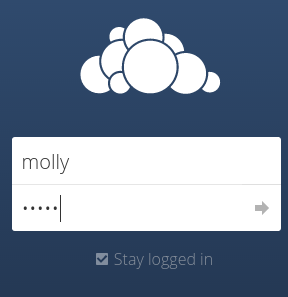
\includegraphics{oc_connect.png}
\end{figure}

\end{itemize}

\begin{notice}{note}{Note:}
Some apps like \code{files\_external} or \code{encryption} will disable
the \textbf{Stay logged in} checkbox.
\end{notice}


\section{Navigating the Main User Interface}
\label{webinterface:navigating-the-main-user-interface}
By default, the ownCloud Web interface opens to your Files page. You can add,
remove, and share files, and make changes based on the access privileges set by
you (if you are administering the server) or by your server administrator.
\begin{figure}[htbp]
\centering

\scalebox{0.750000}{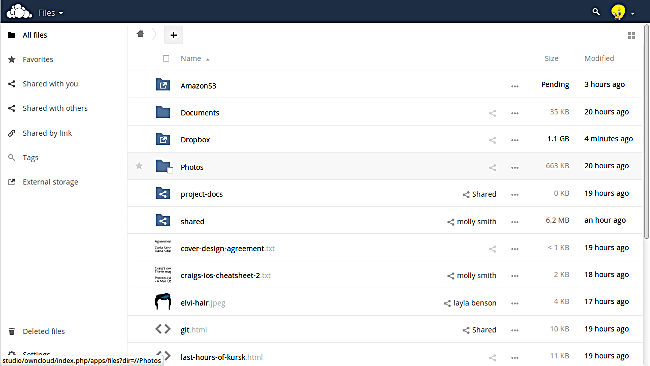
\includegraphics{files_page1.png}}
\end{figure}

The ownCloud user interface contains the following fields and functions:
\begin{itemize}
\item {} 
\textbf{Apps Selection Menu}: Located in the upper left corner, click the arrow to
open a dropdown menu to navigate to your various available apps.

\item {} 
\textbf{Apps Information} field: Located in the left sidebar, this provides
filters and tasks associated with your selected app.  For example, when you
are using the Files apps you have a special set of filters for quickly
finding your files, such as files that have been shared with you, and files
that you have shared with others. You'll see different items for other apps.

\item {} 
\textbf{Application View}: The main central field in the ownCloud user interface.
This field displays the contents or user features of your selected app.

\item {} 
\textbf{Navigation Bar}: Located over the main viewing window (the Application
View), this bar provides a type of breadcrumbs navigation that enables you to
migrate to higher levels of the folder hierarchy up to the root level (home).

\item {} 
\textbf{New} button: Located in the Navigation Bar, the \code{New} button
enables you to create new files, new folders, or upload files.

\end{itemize}

\begin{notice}{note}{Note:}
You can also drag and drop files from your file manager into the
ownCloud Files Application View to upload them to ownCloud. Currently,
the only Web browsers that support drag-and-drop folders are Chrome and
Chromium.
\end{notice}
\begin{itemize}
\item {} 
\textbf{Search} field: Click on the magnifier in the upper right hand corner of
to search for files.

\item {} 
\textbf{Gallery} button. This looks like four little squares, and takes you
directly to your image gallery.

\item {} 
\textbf{Personal Settings} menu: Click on your ownCloud username, located to the
right of the Search field, to open your Personal Settings dropdown menu. Your
Personal page provides the following settings and features:
\begin{itemize}
\item {} 
Links to download desktop and mobile apps

\item {} 
Re-run the First Run Wizard

\item {} 
Server usage and space availability

\item {} 
Password management

\item {} 
Name, email, and profile picture settings

\item {} 
Manage connected browsers and devices

\item {} 
Group memberships

\item {} 
Interface language settings

\item {} 
Manage notifications

\item {} 
Federated Cloud ID

\item {} 
Social media sharing buttons

\item {} 
SSL certificate manager

\item {} 
ownCloud Version information

\end{itemize}

\end{itemize}

See {\hyperref[userpreferences::doc]{\emph{Setting Your Preferences}}} section to learn more about these settings.


\chapter{Files \& Synchronization}
\label{files/index:files-synchronization}\label{files/index::doc}

\section{Accessing your Files Using the ownCloud Web Interface}
\label{files/access_webgui::doc}\label{files/access_webgui:accessing-your-files-using-the-owncloud-web-interface}
You can access your ownCloud files with the ownCloud Web interface and create,
preview, edit, delete, share, and re-share files. Your ownCloud administrator
has the option to disable these features, so if any of them are missing on your
system ask your server administrator.
\begin{figure}[htbp]
\centering

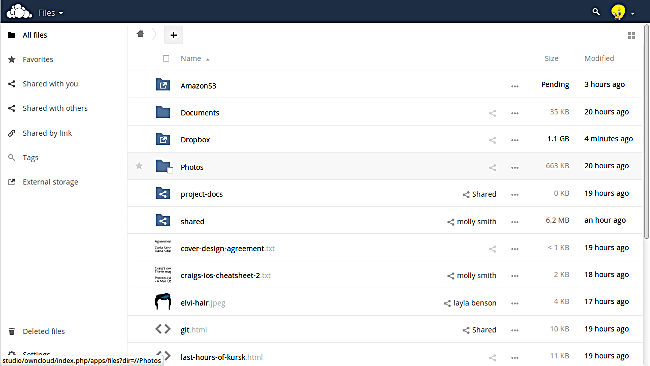
\includegraphics{files_page.png}
\end{figure}


\subsection{Folder Permalinks}
\label{files/access_webgui:folder-permalinks}
Click the share icon on any folder to open the details window on the right. At the top next to the file or folder name click the little chain link icon to expose a permalink. You can give this permalink to any users on your ownCloud server that you have shared the file or folder with. The link remains valid even if the file is renamed.
\begin{figure}[htbp]
\centering

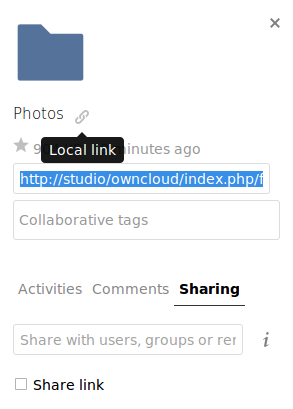
\includegraphics{permalink.png}
\end{figure}


\subsection{Tagging Files}
\label{files/access_webgui:tagging-files}
You can assign tags to files. To create tags, open a file to the Details view.
Then type your tag name. To enter more than one tag press the return key after
creating each tag. All tags are system tags, and are shared by all users on your
ownCloud server.
\begin{figure}[htbp]
\centering

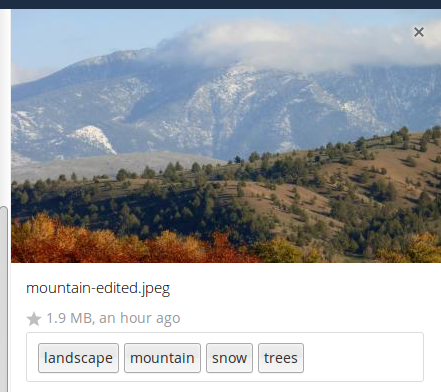
\includegraphics{files_page-7.png}
\end{figure}

Then use the \textbf{Tags} filter on the left sidebar of your Files page to filter files by tags. There are three types of tags:

\textbf{Visible} means that all users may see, rename, and apply these tags to files and folders.

\textbf{Restricted} means tags are assignable and editable only to the user groups have permission to use them. Other users can filter files by restricted tags, but cannot tag files with them or rename them. The tags are marked (restricted).

\textbf{Invisible} means visible only to ownCloud admins.

When you use the \textbf{Tag} filter on your Files page you'll see something like the following image. If you do not have Admin rights then you will not see any invisible tags.
\begin{figure}[htbp]
\centering

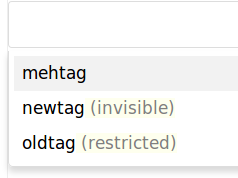
\includegraphics{files_page-8.png}
\end{figure}


\subsection{Comments}
\label{files/access_webgui:comments}
Use the Details view to add and read comments on any file or folder. Comments
are visible to everyone who has access to the file.
\begin{figure}[htbp]
\centering

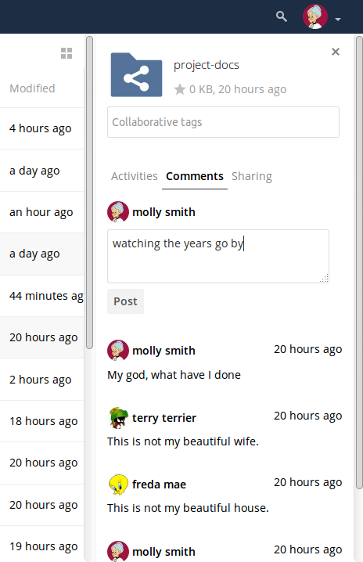
\includegraphics{file_menu_comments_2.png}
\end{figure}


\subsection{Video Player}
\label{files/access_webgui:video-player}
You can play videos in ownCloud with the Video Player app by simply clicking on
the file. Video streaming by the native ownCloud video player depends on your Web browser
and the video format. If your ownCloud administrator has enabled video
streaming, and it doesn't work in your Web browser, it may be a browser issue. See \href{https://developer.mozilla.org/en-US/docs/Web/HTML/Supported\_media\_formats\#Browser\_compatibility}{https://developer.mozilla.org/en-US/docs/Web/HTML/Supported\_media\_formats\#Browser\_compatibility} for supported multimedia formats in Web browsers.
\begin{figure}[htbp]
\centering

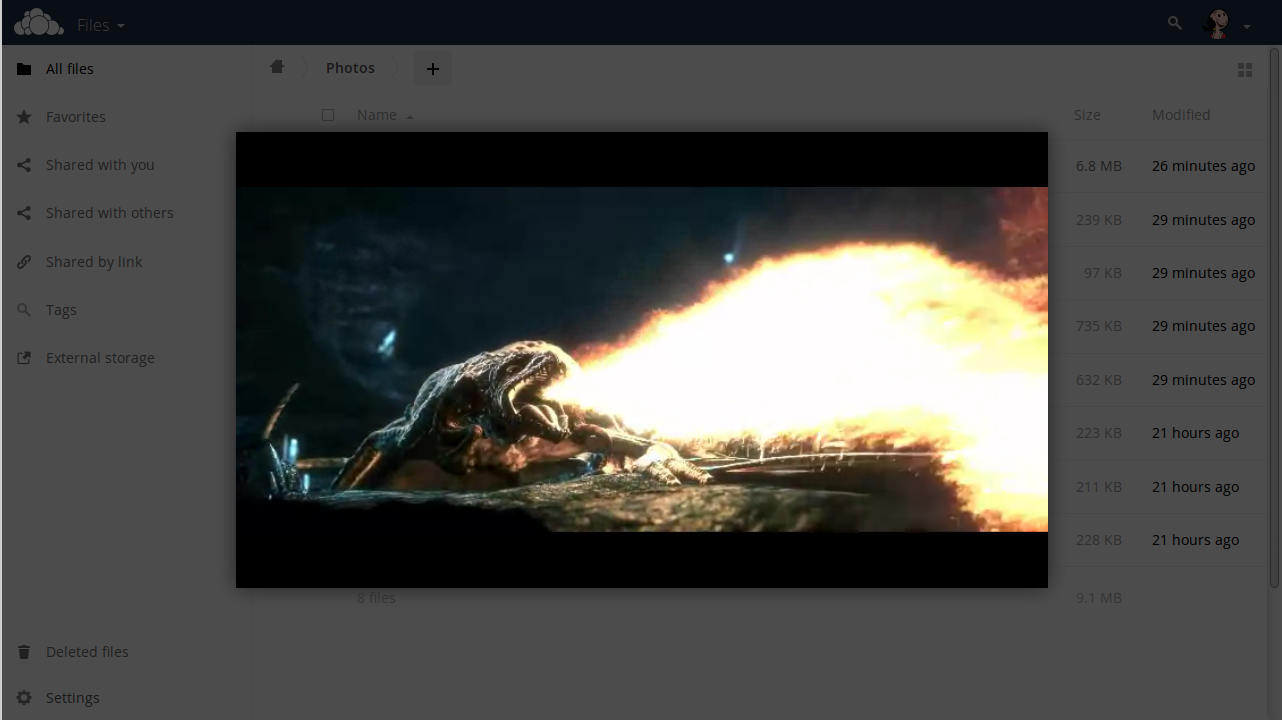
\includegraphics{video_player_2.png}
\end{figure}


\subsection{File Controls}
\label{files/access_webgui:file-controls}
ownCloud can display thumbnail previews for image files, MP3 covers,
and text files, if this enabled by your server administrator. Hover your cursor
over a file or folder to expose the controls for the following operations:
\begin{description}
\item[{Favorites}] \leavevmode
Click the star to the left of the file icon to mark it as a favorite, and
quickly find all of your favorites with the Favorites filter on the left
sidebar.

\end{description}
\begin{figure}[htbp]
\centering

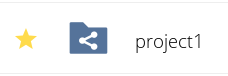
\includegraphics{files_page-1.png}
\end{figure}
\begin{description}
\item[{Share}] \leavevmode
Share the file or folder with a group or other users, and create public
shares with hyperlinks. You can also see who you have shared with already,
and revoke shares by clicking the trash can icon.

\end{description}

\begin{notice}{note}{Note:}
New in 9.0, you can see all re-shares of your original file shares.

If username auto-completion
is enabled, when you start typing the user or group name ownCloud will
automatically complete it for you. If your administrator has enabled email
notifications, you can send an email notification of the new share from the
sharing screen.
\end{notice}
\begin{figure}[htbp]
\centering

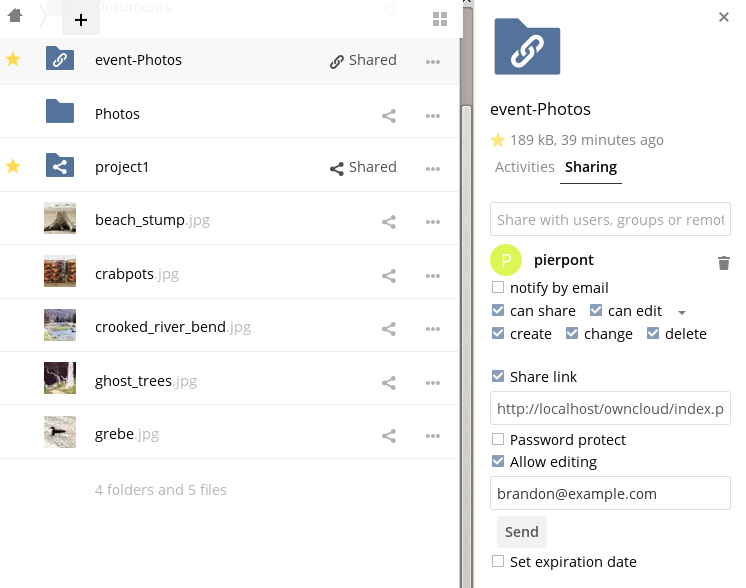
\includegraphics{files_page-2.png}
\end{figure}

You have five share permissions:
\begin{itemize}
\item {} 
Can share; allows the users you share with to re-share.

\item {} 
Can edit; allows the users you share with to edit your shared files, and to collaborate using the Documents app.

\item {} 
Create; allows the users you share with to create new files and add them to the share.

\item {} 
Change; allows uploading a new version of a shared file and replacing it.

\item {} 
Delete; allows the users you share with to delete shared files.

\end{itemize}
\begin{description}
\item[{Overflow Menu}] \leavevmode
The Overflow menu (three dots) displays file details, and allows you to
rename, download, or delete files.

\end{description}
\begin{figure}[htbp]
\centering
\capstart

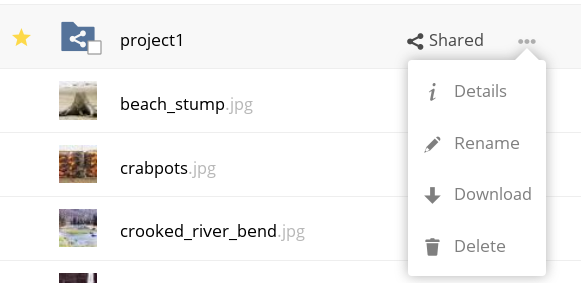
\includegraphics{files_page-3.png}
\caption{The Details view shows Activities, Sharing, and Versions information.}\end{figure}
\begin{figure}[htbp]
\centering

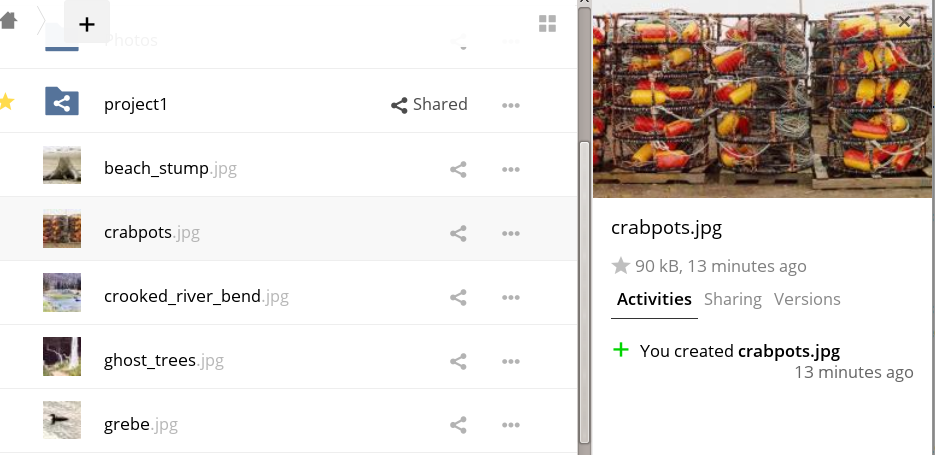
\includegraphics{files_page-4.png}
\end{figure}

The \textbf{Settings} gear icon at the lower left allows you to show or hide hidden
files in your ownCloud Web interface. These are also called dotfiles, because
they are prefixed with a dot, e.g. \code{.mailfile}. The dot tells your operating
system to hide these files in your file browsers, unless you choose to display
them. Usually these are configuration files, so having the option to hide them
reduces clutter.
\begin{figure}[htbp]
\centering

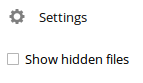
\includegraphics{hidden_files.png}
\end{figure}


\subsection{Previewing Files}
\label{files/access_webgui:previewing-files}
You can display uncompressed text files, OpenDocument files, videos, and image
files in the ownCloud embedded viewers by clicking on the file name. There may
be other file types you can preview if your ownCloud administrator has enabled
them. If ownCloud cannot display a file, it starts a download process and
downloads the file to your computer.


\subsection{Navigating Inside Your ownCloud}
\label{files/access_webgui:navigating-inside-your-owncloud}
Navigating through folders in ownCloud is as simple as clicking on a folder to
open it and using the back button on your browser to move to a previous level.
ownCloud also provides a navigation bar at the top of the Files field for quick
navigation.


\subsection{Sharing Status Icons}
\label{files/access_webgui:sharing-status-icons}
Any folder that has been shared is marked with the \code{Shared} overlay icon.
Public link shares are marked with a chain link. Un-shared folders are blank.
\begin{figure}[htbp]
\centering

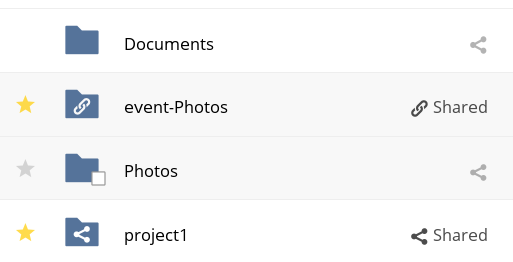
\includegraphics{files_page-5.png}
\end{figure}

If your ownCloud server is the Enterprise edition, you may also have access
to Sharepoint and Windows Network Drive file shares. These have special status
icons. An icon with a red plugin and background means you have to enter a login
to get access to the share.
\begin{figure}[htbp]
\centering

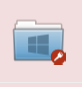
\includegraphics{users-overlays-win-net-drive.png}
\end{figure}
\begin{figure}[htbp]
\centering

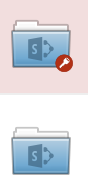
\includegraphics{users-overlays-sharepoint.png}
\end{figure}


\subsection{Creating or Uploading Files and Directories}
\label{files/access_webgui:creating-or-uploading-files-and-directories}
Upload or create new files or folders directly in an ownCloud folder by clicking
on the \emph{New} button in the Files app.
\begin{figure}[htbp]
\centering

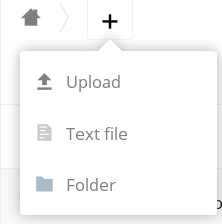
\includegraphics{files_page-6.png}
\end{figure}

The \emph{New} button provides the following options:
\begin{description}
\item[{Up arrow}] \leavevmode
Upload files from your computer into ownCloud. You can also upload files by
dragging and dropping them from your file manager.

\item[{Text file}] \leavevmode
Creates a new text file and adds the file to your current folder.

\item[{Folder}] \leavevmode
Creates a new folder in the current folder.

\end{description}


\subsection{Selecting Files or Folders}
\label{files/access_webgui:selecting-files-or-folders}
You can select one or more files or folders by clicking on their checkboxes.  To
select all files in the current directory, click on the checkbox located at the
top of the files listing.

When you select multiple files, you can delete all of them, or download them as
a ZIP file by using the \code{Delete} or \code{Download} buttons that appear at the
top.

\begin{notice}{note}{Note:}
If the \code{Download} button is not visible, the administrator has
disabled this feature.
\end{notice}


\subsection{Filtering the Files View}
\label{files/access_webgui:filtering-the-files-view}
The right sidebar on the Files page contains several filters for quickly sorting
and managing your files.
\begin{description}
\item[{All files}] \leavevmode
The default view; displays all files that you have access to.

\item[{Favorites}] \leavevmode
Files or folders marked with the yellow star.

\item[{Shared with you}] \leavevmode
Displays all files shared with you by another user or group.

\item[{Shared with others}] \leavevmode
Displays all files that you have shared with other users or groups.

\item[{Shared by link}] \leavevmode
Displays all files that are shared by you via public link.

\item[{External Storage}] \leavevmode
Files that you have access to on external storage devices and services such
as Dropbox, Google, and Amazon S3.

\end{description}


\subsection{Moving Files}
\label{files/access_webgui:moving-files}
You can move files and folders by dragging and dropping them into any directory.


\subsection{Change in Share Expiration Date}
\label{files/access_webgui:change-in-share-expiration-date}
In older versions of ownCloud, you could set an expiration date on both local
and public shares. Now you can set an expiration date only on public shares,
and local shares do not expire when public shares expire. The only way to
``expire'' a local share is to click the trash can icon to un-share your files.


\subsection{Creating or Connecting to a Federation Share Link}
\label{files/access_webgui:creating-or-connecting-to-a-federation-share-link}
Federated Cloud Sharing allows you to mount file shares from remote ownCloud
servers, and manage them just like a local share. In ownCloud 8 the process for
creating a new sharing link is easier and more streamlined. See
{\hyperref[files/federated_cloud_sharing::doc]{\emph{Using Federation Shares}}} to learn to how to create and connect to new
Federated Cloud shares.


\section{Accessing ownCloud Files Using WebDAV}
\label{files/access_webdav:accessing-owncloud-files-using-webdav}\label{files/access_webdav::doc}
ownCloud fully supports the WebDAV protocol, and you can connect and synchronize
with your ownCloud files over WebDAV.  In this chapter you will learn how to
connect Linux, Mac OS X, Windows, and mobile devices to your ownCloud server via
WebDAV. Before we get into configuring WebDAV, let's take a quick look at the
recommended way of connecting client devices to your ownCloud servers.


\subsection{ownCloud Desktop and Mobile Clients}
\label{files/access_webdav:owncloud-desktop-and-mobile-clients}
The recommended method for keeping your desktop PC synchronized with your
ownCloud server is by using the \href{https://owncloud.org/install/\#install-clients}{ownCloud Desktop Client}. You can configure the ownCloud client
to save files in any local directory you want, and you choose which directories
on the ownCloud server to sync with. The client displays the current connection
status and logs all activity, so you always know which remote files have been
downloaded to your PC, and you can verify that files created and updated on your
local PC are properly synchronized with the server.

The recommended method for syncing your ownCloud server with Android and
Apple iOS devices is by using the \href{https://owncloud.org/install/\#install-clients}{ownCloud mobile apps}.

To connect to your ownCloud server with the \textbf{ownCloud} mobile apps, use the
base URL and folder only:

\begin{Verbatim}[commandchars=\\\{\}]
\PYG{n}{example}\PYG{o}{.}\PYG{n}{com}\PYG{o}{/}\PYG{n}{owncloud}
\end{Verbatim}

In addition to the mobile apps provided by ownCloud, you can use other apps to
connect to ownCloud from your mobile device using WebDAV. \href{http://seanashton.net/webdav/}{WebDAV Navigator} is
a good (proprietary) app for \href{https://play.google.com/store/apps/details?id=com.schimera.webdavnavlite}{Android devices}, \href{https://itunes.apple.com/app/webdav-navigator/id382551345}{iPhones}, and \href{http://appworld.blackberry.com/webstore/content/46816}{BlackBerry
devices}. The URL to use on these is:

\begin{Verbatim}[commandchars=\\\{\}]
example.com/owncloud/remote.php/dav/files/USERNAME/
\end{Verbatim}


\subsection{WebDAV Configuration}
\label{files/access_webdav:webdav-configuration}
If you prefer, you may also connect your desktop PC to your ownCloud server by
using the WebDAV protocol rather than using a special client application. Web
Distributed Authoring and Versioning (WebDAV) is a Hypertext Transfer Protocol
(HTTP) extension that makes it easy to create, read, and edit files on Web
servers. With WebDAV you can access your ownCloud shares on Linux, Mac OS X and
Windows in the same way as any remote network share, and stay synchronized.

\begin{notice}{note}{Note:}
In the following examples, You must adjust \textbf{example.com/} to the
URL of your ownCloud server installation.
\end{notice}


\subsection{Accessing Files Using Linux}
\label{files/access_webdav:accessing-files-using-linux}
You can access files in Linux operating systems using the following methods.


\subsubsection{Nautilus File Manager}
\label{files/access_webdav:nautilus-file-manager}
Use the \code{davs://} protocol to connect the Nautilus file manager to your
ownCloud share:

\begin{Verbatim}[commandchars=\\\{\}]
davs://example.com/owncloud/remote.php/dav/files/USERNAME/
\end{Verbatim}

\begin{notice}{note}{Note:}
If your server connection is not HTTPS-secured, use \emph{dav://} instead
of \emph{davs://}.
\end{notice}

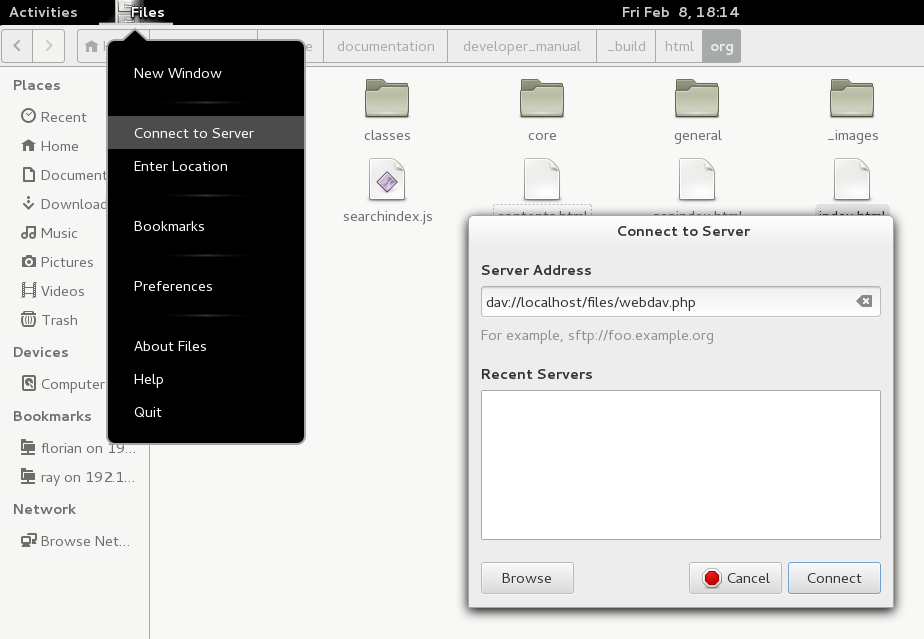
\includegraphics{webdav_gnome3_nautilus.png}


\subsubsection{Accessing Files with KDE and Dolphin File Manager}
\label{files/access_webdav:accessing-files-with-kde-and-dolphin-file-manager}
To access your ownCloud files using the Dolphin file manager in KDE, use
the \code{webdav://} protocol:

\begin{Verbatim}[commandchars=\\\{\}]
webdav://example.com/owncloud/remote.php/dav/files/USERNAME/
\end{Verbatim}

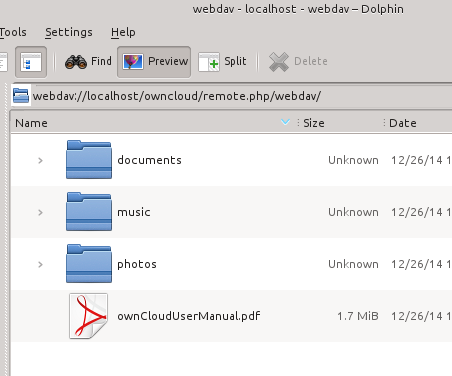
\includegraphics{webdav_dolphin.png}

You can create a permanent link to your ownCloud server:
\begin{enumerate}
\item {} 
Open Dolphin and click ``Network'' in the left hand ``Places'' column.

\item {} 
Click on the icon labeled \textbf{Add a Network Folder}.
The resulting dialog should appear with WebDAV already selected.

\item {} 
If WebDAV is not selected, select it.

\item {} 
Click \textbf{Next}.

\item {} 
Enter the following settings:
\begin{itemize}
\item {} 
Name: The name you want to see in the \textbf{Places} bookmark, for example ownCloud.

\item {} 
User: The ownCloud username you used to log in, for example admin.

\item {} 
Server: The ownCloud domain name, for example \textbf{example.com} (without
\textbf{http://} before or directories afterwards).

\item {} 
Folder -- Enter the path \code{owncloud/remote.php/dav/files/USERNAME/}.

\end{itemize}

\item {} 
(Optional) Check the ``Create icon checkbox'' for a bookmark to appear in the
Places column.

\item {} 
(Optional) Provide any special settings or an SSL certificate in the ``Port \&
Encrypted'' checkbox.

\end{enumerate}


\subsection{Creating WebDAV Mounts on the Linux Command Line}
\label{files/access_webdav:creating-webdav-mounts-on-the-linux-command-line}
You can create WebDAV mounts from the Linux command line. This is useful if you
prefer to access ownCloud the same way as any other remote filesystem mount.
The following example shows how to create a personal mount and have it mounted
automatically every time you log in to your Linux computer.
\begin{enumerate}
\item {} 
Install the \code{davfs2} WebDAV filesystem driver, which allows you to mount
WebDAV shares just like any other remote filesystem. Use this command to
install it on Debian/Ubuntu:

\begin{Verbatim}[commandchars=\\\{\}]
apt\PYGZhy{}get install davfs2
\end{Verbatim}

\item {} 
Use this command to install it on CentOS, Fedora, and openSUSE:

\begin{Verbatim}[commandchars=\\\{\}]
yum install davfs2
\end{Verbatim}

\item {} 
Add yourself to the \code{davfs2} group:

\begin{Verbatim}[commandchars=\\\{\}]
usermod \PYGZhy{}aG davfs2 \PYGZlt{}username\PYGZgt{}
\end{Verbatim}

\end{enumerate}
\begin{enumerate}
\setcounter{enumi}{2}
\item {} 
Then create an \code{owncloud} directory in your home directory for the
mountpoint, and \code{.davfs2/} for your personal configuration file:

\begin{Verbatim}[commandchars=\\\{\}]
mkdir \PYGZti{}/owncloud
mkdir \PYGZti{}/.davfs2
\end{Verbatim}

\item {} 
Copy \code{/etc/davfs2/secrets} to \code{\textasciitilde{}/.davfs2}:

\begin{Verbatim}[commandchars=\\\{\}]
cp  /etc/davfs2/secrets \PYGZti{}/.davfs2/secrets
\end{Verbatim}

\item {} 
Set yourself as the owner and make the permissions read-write owner only:

\begin{Verbatim}[commandchars=\\\{\}]
chown \PYGZlt{}username\PYGZgt{}:\PYGZlt{}username\PYGZgt{}  \PYGZti{}/.davfs2/secrets
chmod 600 \PYGZti{}/.davfs2/secrets
\end{Verbatim}

\item {} 
Add your ownCloud login credentials to the end of the \code{secrets} file,
using your ownCloud server URL and your ownCloud username and password:

\begin{Verbatim}[commandchars=\\\{\}]
example.com/owncloud/remote.php/dav/files/USERNAME/ \PYGZlt{}username\PYGZgt{} \PYGZlt{}password\PYGZgt{}
\end{Verbatim}

\item {} 
Add the mount information to \code{/etc/fstab}:

\begin{Verbatim}[commandchars=\\\{\}]
example.com/owncloud/remote.php/dav/files/USERNAME/ /home/\PYGZlt{}username\PYGZgt{}/owncloud
davfs user,rw,auto 0 0
\end{Verbatim}

\item {} 
Then test that it mounts and authenticates by running the following
command. If you set it up correctly you won't need root permissions:

\begin{Verbatim}[commandchars=\\\{\}]
mount \PYGZti{}/owncloud
\end{Verbatim}

\item {} 
You should also be able to unmount it:

\begin{Verbatim}[commandchars=\\\{\}]
umount \PYGZti{}/owncloud
\end{Verbatim}

\end{enumerate}

Now every time you login to your Linux system your ownCloud share should
automatically mount via WebDAV in your \code{\textasciitilde{}/owncloud} directory. If you prefer
to mount it manually, change \code{auto} to \code{noauto} in \code{/etc/fstab}.


\subsection{Known Issues}
\label{files/access_webdav:known-issues}

\subsubsection{Problem}
\label{files/access_webdav:problem}
Resource temporarily unavailable


\subsubsection{Solution}
\label{files/access_webdav:solution}
If you experience trouble when you create a file in the directory,
edit \code{/etc/davfs2/davfs2.conf} and add:

\begin{Verbatim}[commandchars=\\\{\}]
use\PYGZus{}locks 0
\end{Verbatim}


\subsubsection{Problem}
\label{files/access_webdav:id1}
Certificate warnings


\subsubsection{Solution}
\label{files/access_webdav:id2}
If you use a self-signed certificate, you will get a warning. To
change this, you need to configure \code{davfs2} to recognize your certificate.
Copy \code{mycertificate.pem} to \code{/etc/davfs2/certs/}. Then edit
\code{/etc/davfs2/davfs2.conf} and uncomment the line \code{servercert}. Now add the
path of your certificate as in this example:

\begin{Verbatim}[commandchars=\\\{\}]
\PYG{n}{servercert}   \PYG{o}{/}\PYG{n}{etc}\PYG{o}{/}\PYG{n}{davfs2}\PYG{o}{/}\PYG{n}{certs}\PYG{o}{/}\PYG{n}{mycertificate}\PYG{o}{.}\PYG{n}{pem}
\end{Verbatim}


\subsection{Accessing Files Using Mac OS X}
\label{files/access_webdav:accessing-files-using-mac-os-x}
\begin{notice}{note}{Note:}
The Mac OS X Finder suffers from a \href{http://sabre.io/dav/clients/finder/}{series of implementation problems} and should only be used if the
ownCloud server runs on \textbf{Apache} and \textbf{mod\_php}, or \textbf{Nginx 1.3.8+}.
\end{notice}

To access files through the Mac OS X Finder:
\begin{enumerate}
\item {} 
Choose \textbf{Go \textgreater{} Connect to Server}.

\end{enumerate}
\begin{quote}

The ``Connect to Server'' window opens.
\end{quote}
\begin{enumerate}
\setcounter{enumi}{1}
\item {} 
Specify the address of the server in the \textbf{Server Address} field.

\end{enumerate}
\begin{quote}

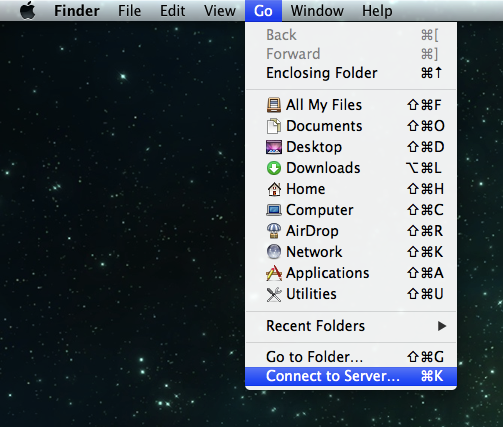
\includegraphics{osx_webdav1.png}

For example, the URL used to connect to the ownCloud server
from the Mac OS X Finder is:

\begin{Verbatim}[commandchars=\\\{\}]
https://example.com/owncloud/remote.php/dav/files/USERNAME/
\end{Verbatim}

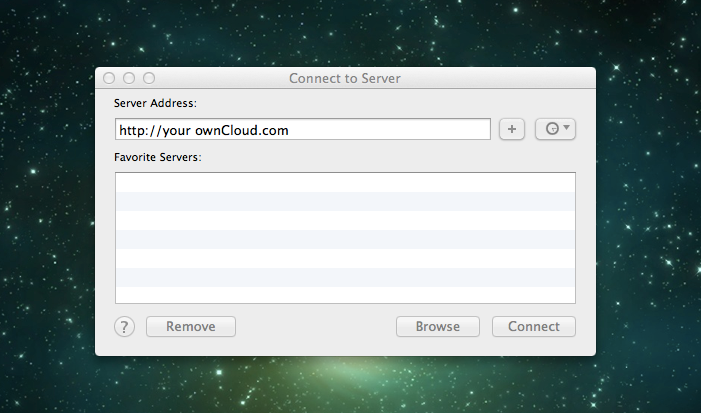
\includegraphics{osx_webdav2.png}
\end{quote}
\begin{enumerate}
\setcounter{enumi}{2}
\item {} 
Click \textbf{Connect}.

\end{enumerate}
\begin{quote}

The device connects to the server.
\end{quote}

For added details about how to connect to an external server using Mac OS X,
check the \href{http://docs.info.apple.com/article.html?path=Mac/10.6/en/8160.html}{vendor documentation}


\subsection{Accessing Files Using Microsoft Windows}
\label{files/access_webdav:accessing-files-using-microsoft-windows}
It is best to use a suitable WebDAV client from the
\href{http://www.webdav.org/projects/}{WebDAV Project page} .

If you must use the native Windows implementation, you can map ownCloud to a new
drive. Mapping to a drive enables you to browse files stored on an ownCloud
server the way you would files stored in a mapped network drive.

Using this feature requires network connectivity. If you want to store your
files offline, use the ownCloud Desktop Client to sync all files on your
ownCloud to one or more directories of your local hard drive.

\begin{notice}{note}{Note:}
Prior to mapping your drive, you must permit the use of Basic
Authentication in the Windows Registry. The procedure is documented in
\href{http://support.microsoft.com/kb/841215}{KB841215} and differs between Windows XP/Server 2003 and Windows Vista/7.
Please follow the Knowledge Base article before proceeding, and follow the
Vista instructions if you run Windows 7.
\end{notice}


\subsubsection{Mapping Drives With the Command Line}
\label{files/access_webdav:kb841215}\label{files/access_webdav:mapping-drives-with-the-command-line}
The following example shows how to map a drive using the command line.  To map
the drive:
\begin{enumerate}
\item {} 
Open a command prompt in Windows.

\item {} 
Enter the following line in the command prompt to map to the computer Z
drive:

\begin{Verbatim}[commandchars=\\\{\}]
net use Z: https://\PYGZlt{}drive\PYGZus{}path\PYGZgt{}/remote.php/dav/files/USERNAME/ /user:youruser
yourpassword
\end{Verbatim}

\end{enumerate}
\begin{quote}

where \textless{}drive\_path\textgreater{} is the URL to your ownCloud server.
\end{quote}

For example: \code{net use Z: https://example.com/owncloud/remote.php/dav/files/USERNAME/
/user:youruser yourpassword}
\begin{quote}

The computer maps the files of your ownCloud account to the drive letter Z.
\end{quote}

\begin{notice}{note}{Note:}
Though not recommended, you can also mount the ownCloud server
using HTTP, leaving the connection unencrypted.  If you plan to use HTTP
connections on devices while in a public place, we strongly recommend using a
VPN tunnel to provide the necessary security.
\end{notice}

An alternative command syntax is:

\begin{Verbatim}[commandchars=\\\{\}]
net use Z: \PYGZbs{}\PYGZbs{}example.com@ssl\PYGZbs{}owncloud\PYGZbs{}remote.php\PYGZbs{}dav /user:youruser
yourpassword
\end{Verbatim}


\subsubsection{Mapping Drives With Windows Explorer}
\label{files/access_webdav:mapping-drives-with-windows-explorer}
To map a drive using the Microsoft Windows Explorer:
\begin{enumerate}
\item {} 
Migrate to your computer in Windows Explorer.

\item {} 
Right-click on \textbf{Computer} entry and select \textbf{Map network drive...} from
the drop-down menu.

\item {} 
Choose a local network drive to which you want to map ownCloud.

\item {} 
Specify the address to your ownCloud instance, followed by
\textbf{/remote.php/dav/files/USERNAME/}.

\end{enumerate}
\begin{quote}

For example:

\begin{Verbatim}[commandchars=\\\{\}]
https://example.com/owncloud/remote.php/dav/files/USERNAME/
\end{Verbatim}
\end{quote}

\begin{notice}{note}{Note:}
For SSL protected servers, check \textbf{Reconnect at logon} to ensure
that the mapping is persistent upon subsequent reboots. If you want to
connect to the ownCloud server as a different user, check \textbf{Connect using
different credentials}.
\end{notice}
\begin{figure}[htbp]
\centering

\scalebox{0.800000}{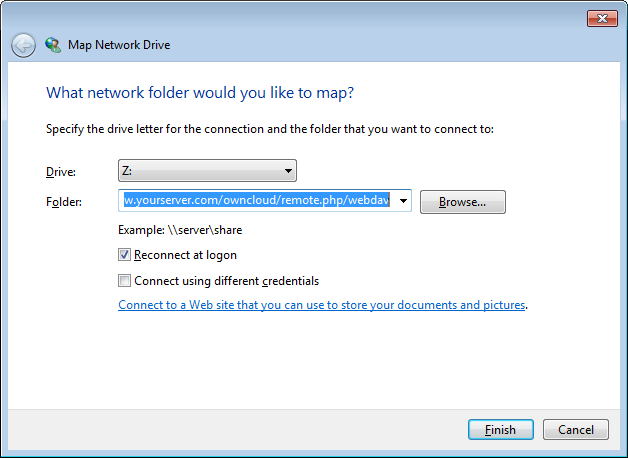
\includegraphics{explorer_webdav.png}}
\end{figure}
\begin{enumerate}
\setcounter{enumi}{4}
\item {} 
Click the \code{Finish} button.

\end{enumerate}
\begin{quote}

Windows Explorer maps the network drive, making your ownCloud instance
available.
\end{quote}


\subsection{Accessing Files Using Cyberduck}
\label{files/access_webdav:accessing-files-using-cyberduck}
\href{https://cyberduck.io/?l=en}{Cyberduck} is an open source FTP and SFTP,
WebDAV, OpenStack Swift, and Amazon S3 browser designed for file transfers on
Mac OS X and Windows.

\begin{notice}{note}{Note:}
This example uses Cyberduck version 4.2.1.
\end{notice}

To use Cyberduck:
\begin{enumerate}
\item {} 
Specify a server without any leading protocol information. For example:

\end{enumerate}
\begin{quote}

\code{example.com}
\end{quote}

2. Specify the appropriate port.  The port you choose depends on whether or not
your ownCloud server supports SSL. Cyberduck requires that you select a
different connection type if you plan to use SSL.  For example:
\begin{quote}

80 (for WebDAV)

443 (for WebDAV (HTTPS/SSL))
\end{quote}

3. Use the `More Options' drop-down menu to add the rest of your WebDAV URL into
the `Path' field. For example:
\begin{quote}

\code{remote.php/dav/files/USERNAME/}
\end{quote}

Now Cyberduck enables file access to the ownCloud server.


\subsection{Accessing public shares over WebDAV}
\label{files/access_webdav:accessing-public-shares-over-webdav}
ownCloud provides the possibility to access public shares over WebDAV.

To access the public share, open:

\begin{Verbatim}[commandchars=\\\{\}]
https://example.com/owncloud/public.php/dav
\end{Verbatim}

in a WebDAV client, use the share token as username and the (optional) share password
as password.


\subsection{Known Problems}
\label{files/access_webdav:known-problems}

\subsubsection{Problem}
\label{files/access_webdav:id3}
Windows does not connect using HTTPS.


\subsubsection{Solution 1}
\label{files/access_webdav:solution-1}
The Windows WebDAV Client might not support Server Name Indication (SNI) on
encrypted connections. If you encounter an error mounting an SSL-encrypted
ownCloud instance, contact your provider about assigning a dedicated IP address
for your SSL-based server.


\subsubsection{Solution 2}
\label{files/access_webdav:solution-2}
The Windows WebDAV Client might not support TSLv1.1 / TSLv1.2 connections. If
you have restricted your server config to only provide TLSv1.1 and above the
connection to your server might fail. Please refer to the \href{https://msdn.microsoft.com/en-us/library/windows/desktop/aa382925.aspx\#WinHTTP\_5.1\_Features}{WinHTTP} documentation
for further information.


\subsubsection{Problem}
\label{files/access_webdav:id4}\label{files/access_webdav:winhttp}
You receive the following error message: \textbf{Error 0x800700DF: The file size
exceeds the limit allowed and cannot be saved.}


\subsubsection{Solution}
\label{files/access_webdav:id5}
Windows limits the maximum size a file transferred from or to  a WebDAV share
may have.  You can increase the value \textbf{FileSizeLimitInBytes} in
\textbf{HKEY\_LOCAL\_MacHINE\textbackslash{}SYSTEM\textbackslash{}CurrentControlSet\textbackslash{}Services\textbackslash{}WebClient\textbackslash{}Parameters
** by clicking on **Modify}.

To increase the limit to the maximum value of 4GB, select \textbf{Decimal}, enter a
value of \textbf{4294967295}, and reboot Windows or restart the \textbf{WebClient}
service.


\subsubsection{Problem}
\label{files/access_webdav:id6}
Accessing your files from Microsoft Office via WebDAV fails.


\subsubsection{Solution}
\label{files/access_webdav:id7}
Known problems and their solutions are documented in the \href{https://support.microsoft.com/kb/2123563}{KB2123563} article.


\subsubsection{Problem}
\label{files/access_webdav:id8}
Cannot map ownCloud as a WebDAV drive in Windows using self-signed certificate.


\subsubsection{Solution}
\label{files/access_webdav:id9}\begin{enumerate}
\item {} 
Go to the your ownCloud instance via your favorite Web browser.

\item {} 
Click through until you get to the certificate error in the browser status
line.

\item {} 
View the cert, then from the Details tab, select Copy to File.

\item {} 
Save to the desktop with an arbitrary name, for example \code{myOwnCloud.cer}.

\item {} 
Start, Run, MMC.

\item {} 
File, Add/Remove Snap-In.

\item {} 
Select Certificates, Click Add, My User Account, then Finish, then OK.

\item {} 
Dig down to Trust Root Certification Authorities, Certificates.

\item {} 
Right-Click Certificate, Select All Tasks, Import.

\item {} 
Select the Save Cert from the Desktop.

\item {} 
Select Place all Certificates in the following Store, Click Browse,

\item {} 
Check the Box that says Show Physical Stores, Expand out Trusted Root
Certification Authorities, and select Local Computer there, click OK,
Complete the Import.

\item {} 
Check the list to make sure it shows up. You will probably need to Refresh
before you see it. Exit MMC.

\item {} 
Open Browser, select Tools, Delete Browsing History.

\item {} 
Select all but In Private Filtering Data, complete.

\item {} 
Go to Internet Options, Content Tab, Clear SSL State.

\item {} 
Close browser, then re-open and test.

\end{enumerate}


\subsubsection{Problem}
\label{files/access_webdav:id10}
You cannot download more than 50 MB or upload large Files when the upload takes
longer than 30 minutes using Web Client in Windows 7.


\subsubsection{Solution}
\label{files/access_webdav:id11}
Workarounds are documented in the \href{https://support.microsoft.com/kb/2668751}{KB2668751} article.


\subsubsection{Problem}
\label{files/access_webdav:id12}
Error 0x80070043 ``The network name cannot be found.'' while adding a network drive.


\subsubsection{Solution}
\label{files/access_webdav:id13}
Make Windows service \textbf{WebClient} start automatically:
\begin{enumerate}
\item {} 
Open \textbf{Control Panel}.

\item {} 
Go to \textbf{Administrative Tools}.

\item {} 
Launch \textbf{Services}.

\item {} 
Find \textbf{WebClient} service.

\item {} 
Right-click on it and choose \textbf{Properties}.

\item {} 
Select \textbf{Startup type}: \textbf{Automatic}.

\item {} 
Click \textbf{OK} button.

\end{enumerate}

Or in command prompt (as Admin):

\begin{Verbatim}[commandchars=\\\{\}]
sc config \PYGZdq{}WebClient\PYGZdq{} start=auto
sc start \PYGZdq{}WebClient\PYGZdq{}
\end{Verbatim}

More details \href{https://github.com/owncloud/documentation/pull/2668}{here}.


\subsection{Accessing Files Using cURL}
\label{files/access_webdav:accessing-files-using-curl}
Since WebDAV is an extension of HTTP cURL can be used to script file operations.

To create a folder with the current date as name:

\begin{Verbatim}[commandchars=\\\{\}]
\PYG{n+nv}{\PYGZdl{} }curl \PYGZhy{}u user:pass \PYGZhy{}X MKCOL \PYG{l+s+s2}{\PYGZdq{}https://example.com/owncloud/remote.php/dav/files/USERNAME/\PYGZdl{}(date \PYGZsq{}+\PYGZpc{}d\PYGZhy{}\PYGZpc{}b\PYGZhy{}\PYGZpc{}Y\PYGZsq{})\PYGZdq{}}
\end{Verbatim}

To upload a file \code{error.log} into that directory:

\begin{Verbatim}[commandchars=\\\{\}]
\PYG{n+nv}{\PYGZdl{} }curl \PYGZhy{}u user:pass \PYGZhy{}T error.log \PYG{l+s+s2}{\PYGZdq{}https://example.com/owncloud/remote.php/dav/files/USERNAME/\PYGZdl{}(date \PYGZsq{}+\PYGZpc{}d\PYGZhy{}\PYGZpc{}b\PYGZhy{}\PYGZpc{}Y\PYGZsq{})/error.log\PYGZdq{}}
\end{Verbatim}

To move a file:

\begin{Verbatim}[commandchars=\\\{\}]
\PYG{n+nv}{\PYGZdl{} }curl \PYGZhy{}u user:pass \PYGZhy{}X MOVE \PYGZhy{}\PYGZhy{}header \PYG{l+s+s1}{\PYGZsq{}Destination: https://example.com/owncloud/remote.php/dav/files/USERNAME/target.jpg\PYGZsq{}} https://example.com/owncloud/remote.php/dav/files/USERNAME/source.jpg
\end{Verbatim}

To get the properties of files in the root folder:

\begin{Verbatim}[commandchars=\\\{\}]
    \PYG{n+nv}{\PYGZdl{} }curl \PYGZhy{}X PROPFIND \PYGZhy{}H \PYG{l+s+s2}{\PYGZdq{}Depth: 1\PYGZdq{}} \PYGZhy{}u user:pass https://example.com/owncloud/remote.php/dav/files/USERNAME/ \textbar{} xml\PYGZus{}pp
    \PYGZlt{}?xml \PYG{n+nv}{version}\PYG{o}{=}\PYG{l+s+s2}{\PYGZdq{}1.0\PYGZdq{}} \PYG{n+nv}{encoding}\PYG{o}{=}\PYG{l+s+s2}{\PYGZdq{}utf\PYGZhy{}8\PYGZdq{}}?\PYGZgt{}
\PYGZlt{}d:multistatus xmlns:d\PYG{o}{=}\PYG{l+s+s2}{\PYGZdq{}DAV:\PYGZdq{}} xmlns:oc\PYG{o}{=}\PYG{l+s+s2}{\PYGZdq{}http://owncloud.org/ns\PYGZdq{}} xmlns:s\PYG{o}{=}\PYG{l+s+s2}{\PYGZdq{}http://sabredav.org/ns\PYGZdq{}}\PYGZgt{}
  \PYGZlt{}d:response\PYGZgt{}
    \PYGZlt{}d:href\PYGZgt{}/owncloud/remote.php/dav/files/USERNAME/\PYGZlt{}/d:href\PYGZgt{}
    \PYGZlt{}d:propstat\PYGZgt{}
      \PYGZlt{}d:prop\PYGZgt{}
        \PYGZlt{}d:getlastmodified\PYGZgt{}Tue, 13 Oct 2015 17:07:45 GMT\PYGZlt{}/d:getlastmodified\PYGZgt{}
        \PYGZlt{}d:resourcetype\PYGZgt{}
          \PYGZlt{}d:collection/\PYGZgt{}
        \PYGZlt{}/d:resourcetype\PYGZgt{}
        \PYGZlt{}d:quota\PYGZhy{}used\PYGZhy{}bytes\PYGZgt{}163\PYGZlt{}/d:quota\PYGZhy{}used\PYGZhy{}bytes\PYGZgt{}
        \PYGZlt{}d:quota\PYGZhy{}available\PYGZhy{}bytes\PYGZgt{}11802275840\PYGZlt{}/d:quota\PYGZhy{}available\PYGZhy{}bytes\PYGZgt{}
        \PYGZlt{}d:getetag\PYGZgt{}\PYG{l+s+s2}{\PYGZdq{}561d3a6139d05\PYGZdq{}}\PYGZlt{}/d:getetag\PYGZgt{}
      \PYGZlt{}/d:prop\PYGZgt{}
      \PYGZlt{}d:status\PYGZgt{}HTTP/1.1 200 OK\PYGZlt{}/d:status\PYGZgt{}
    \PYGZlt{}/d:propstat\PYGZgt{}
  \PYGZlt{}/d:response\PYGZgt{}
  \PYGZlt{}d:response\PYGZgt{}
    \PYGZlt{}d:href\PYGZgt{}/owncloud/remote.php/dav/files/USERNAME/welcome.txt\PYGZlt{}/d:href\PYGZgt{}
    \PYGZlt{}d:propstat\PYGZgt{}
      \PYGZlt{}d:prop\PYGZgt{}
        \PYGZlt{}d:getlastmodified\PYGZgt{}Tue, 13 Oct 2015 17:07:35 GMT\PYGZlt{}/d:getlastmodified\PYGZgt{}
        \PYGZlt{}d:getcontentlength\PYGZgt{}163\PYGZlt{}/d:getcontentlength\PYGZgt{}
        \PYGZlt{}d:resourcetype/\PYGZgt{}
        \PYGZlt{}d:getetag\PYGZgt{}\PYG{l+s+s2}{\PYGZdq{}47465fae667b2d0fee154f5e17d1f0f1\PYGZdq{}}\PYGZlt{}/d:getetag\PYGZgt{}
        \PYGZlt{}d:getcontenttype\PYGZgt{}text/plain\PYGZlt{}/d:getcontenttype\PYGZgt{}
      \PYGZlt{}/d:prop\PYGZgt{}
      \PYGZlt{}d:status\PYGZgt{}HTTP/1.1 200 OK\PYGZlt{}/d:status\PYGZgt{}
    \PYGZlt{}/d:propstat\PYGZgt{}
  \PYGZlt{}/d:response\PYGZgt{}
\PYGZlt{}/d:multistatus\PYGZgt{}
\end{Verbatim}


\section{Gallery App}
\label{files/gallery_app:gallery-app}\label{files/gallery_app::doc}
The Pictures app has been rewritten and improved, and is now called the Gallery
app. It supports more image formats, sorting, zoom, and scrolling. It also
supports advanced customizations via a simple text file.

On your main ownCloud Files page, click the little icon at the top right,
underneath your username, to open your Gallery. The Gallery app automatically
finds all images in your ownCloud folders, and overlays the thumbnails with the
folder names. Click on the folder thumbnails to open the folders. At the top
left you have two sorting options, alphabetical and by date.
\begin{figure}[htbp]
\centering

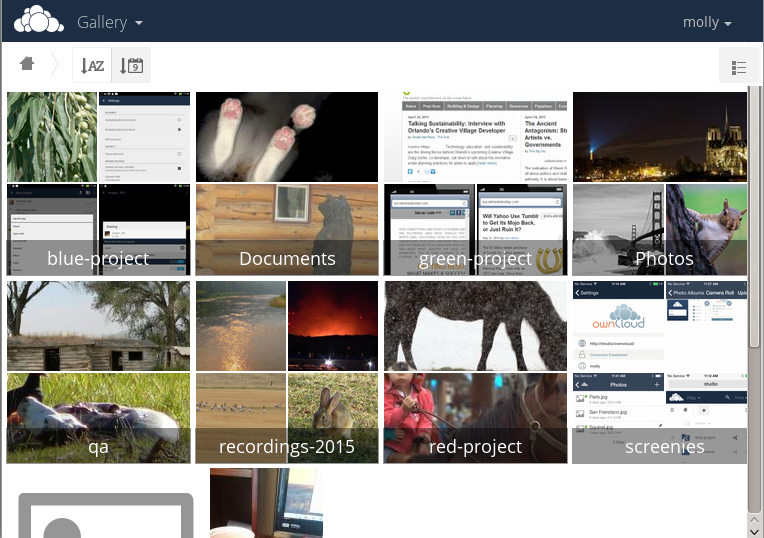
\includegraphics{gallery-1.png}
\end{figure}

After entering any folder, click on any image to open it in slideshow mode.
This has the following features: a download button at the top center, forward
and back buttons at the right and left sides, an automatic slideshow button at
the bottom right, and a close button at the top right.
\begin{figure}[htbp]
\centering

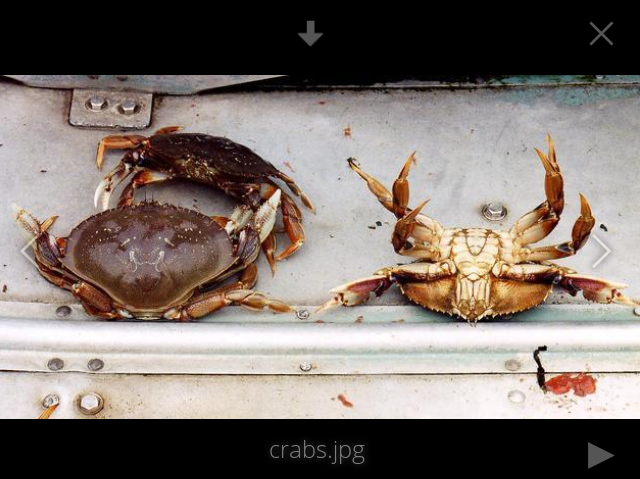
\includegraphics{gallery-2.png}
\end{figure}


\subsection{Custom Configuration}
\label{files/gallery_app:custom-configuration}
You may customize a Gallery album with a simple text file named
\textbf{gallery.cnf}, which contains parameters structured using the
\href{https://en.wikipedia.org/wiki/YAML}{Yaml} markup language. You may have
multiple \textbf{gallery.cnf} files; you need one in your own root ownCloud folder
(your Home folder) that defines global features, and then you may have
individual per-album \textbf{gallery.cnf} files if you want to define different
behaviors in different albums.


\subsubsection{Features}
\label{files/gallery_app:features}
The following general features are currently implemented:
\begin{itemize}
\item {} 
Native SVG support.

\item {} 
Access to external shares.

\end{itemize}

The following album features are currently implemented:
\begin{itemize}
\item {} 
Adding a link to a file containing a description.

\item {} 
Typing a simple copyright statement directly in the configuration file.

\item {} 
Adding a link to a file containing a copyright statement.

\item {} 
Defining a sort type and order.

\item {} 
Defining the colour of the background.

\item {} 
Defining if sub-albums will inherit the configuration.

\end{itemize}

The following slideshow features are currently implemented:
\begin{itemize}
\item {} 
Showing a button which lets you pick which background, either black or
white, to use for the picture you are currently viewing (for images with
transparent backgrounds).

\end{itemize}


\subsubsection{Setup}
\label{files/gallery_app:setup}
The configuration file has to be named \textbf{gallery.cnf}. You may have multiple
per-album \textbf{gallery.cnf} files. To enable global features, place one in your
top-level folder, which is symbolised in the Web GUI by the home icon. (This
puts it in \code{data/\textless{}user\textgreater{}/files/}.) See {\hyperref[files/gallery_app:supported-variables-label]{\emph{an example below}}} in the \textbf{Global features} section.

\begin{notice}{note}{Note:}
You need to refresh your browser after changing your configuration to
see your changes.
\end{notice}


\subsubsection{Format}
\label{files/gallery_app:format}
UTF-8, \textbf{without BOM}. A file created from within the ownCloud Web GUI works.


\subsubsection{Structure}
\label{files/gallery_app:structure}
You should include a comment in the file, so that people stumbling upon
the file know what it's for. Comments start with \#.

Spacing is created using 2 spaces. \textbf{Do not use tabs.}

Take a look at the \href{http://symfony.com/doc/current/components/yaml/yaml\_format.html}{YAML Format documentation} if you are
getting error messages.

Here is an example \emph{gallery.cnf}:

\begin{Verbatim}[commandchars=\\\{\}]
 \PYGZsh{} Gallery configuration file
 \PYGZsh{} Created on 31 Jan 2016 by ownCloud User
features:
  external\PYGZus{}shares: yes
  native\PYGZus{}svg: yes
  background\PYGZus{}colour\PYGZus{}toggle: yes
design:
  background: \PYGZdq{}\PYGZsh{}ff9f00\PYGZdq{}
  inherit: yes
information:
  description: This is an **album description** which is only shown if there
  is no {}`description\PYGZus{}link{}`
  description\PYGZus{}link: readme.md
  copyright: Copyright 2003\PYGZhy{}2016 [interfaSys sàrl](http://www.interfasys.ch),
  Switzerland
  copyright\PYGZus{}link: copyright.md
  inherit: yes
sorting:
  type: date
  order: des
  inherit: yes
\end{Verbatim}


\subsubsection{Supported Variables}
\label{files/gallery_app:supported-variables}\label{files/gallery_app:supported-variables-label}
\textbf{Global Features}

Place this in your root ownCloud folder, which is your Home folder.
\begin{itemize}
\item {} 
\textbf{external\_shares}: Set to \textbf{yes} in your root configuration file if you
want to load images stored on external locations, when using the
\textbf{files\_external} app.

\item {} 
\textbf{native\_svg}: Set to \textbf{yes} in your root configuration file to enable
rendering SVG images in your browser. This may represent a security risk if
you can't fully trust your SVG files.

\item {} 
\textbf{background\_colour\_toggle}: Set to \textbf{yes} in your root configuration file
to enable a button that toggles between black and white backgrounds on
transparent images.

\end{itemize}

\begin{notice}{note}{Note:}
External shares are 20-50 times slower than local shares. Be prepared
to wait a long time before being able to see all the images contained in a
shared album.
\end{notice}

\textbf{Album Configuration}

Each album can be individually configured using the following configuration
sections. Use the \textbf{inherit} parameter to pass configurations on to
sub-albums.

\textbf{Design}
\begin{itemize}
\item {} 
\textbf{background}: Defines the colour of the background of the photowall
using the RGB hexadecimal representation of that colour. For example:
\textbf{``\#ffa033''}. You must use quotes around the value or it will
be ignored. It is strongly recommended to use a custom theme, with a CSS
loading spinner if you intend to use this feature. You can use \href{http://paletton.com/}{this colour
wheel} to find a colour you like.

\item {} 
\textbf{inherit}: Set to \textbf{yes} if you want sub-folders to inherit this part of
the configuration.

\end{itemize}

\textbf{Album Presentation}
\begin{itemize}
\item {} 
\textbf{description}: A markdown-formatted string which will be displayed in the
info box. It can spread over multiple lines using the Yaml markers.

\item {} 
\textbf{description\_link}: A markdown file located within the album which will
be parsed and displayed in the info box instead of the description.

\item {} 
\textbf{copyright}: A markdown-formatted string. This supports links to external
resources.

\item {} 
\textbf{copyright\_link}: Any file (e.g. copyright.html), in the album itself,
which will be downloaded when the user clicks on the link

\item {} 
\textbf{inherit}: Set to \textbf{yes} if you want sub-folders to inherit this part of
the configuration.

\end{itemize}

See \href{http://www.markitdown.net/markdown}{http://www.markitdown.net/markdown} for the markdown syntax.

\begin{notice}{note}{Note:}
Do not add links to your \emph{copyright} string if you use the
\textbf{copyright\_link} variable.
\end{notice}

\textbf{Sorting}
\begin{itemize}
\item {} 
\textbf{sorting}: \textbf{date} or \textbf{name}. \textbf{date} only works for files.

\item {} 
\textbf{sort\_order}: \textbf{asc} or \textbf{des} (Ascending or descending).

\item {} 
\textbf{inherit}: Set to \textbf{yes} if you want sub-folders to inherit this part of
the configuration.

\end{itemize}


\subsection{Notes}
\label{files/gallery_app:notes}\begin{itemize}
\item {} 
When only the sort \textbf{type} variable has been set, the default sort order
will be used.

\item {} 
When only the sort \textbf{order} variable has been found, the sort configuration
will be ignored and the script will keep looking for a valid configuration in
upper folders.

\item {} 
To enable a feature such as native SVG in a public share, you need to create
in that folder a configuration file containing that feature.

\item {} 
If you share a folder publicly, don't forget to add all the files you link to
(e.g. \code{description.md} or \code{copyright.md}) inside the shared folder as
the user won't have access to files stored in the parent folder.

\item {} 
Since people can download a whole folder as an archive, it's usually best to
include all files within a shared folder, rather than adding text directly
in the configuration file.

\end{itemize}


\subsection{Examples}
\label{files/gallery_app:examples}
\textbf{Sorting Only}

Applies to the current folder only:

\begin{Verbatim}[commandchars=\\\{\}]
\PYGZsh{} Gallery configuration file
  sorting:
  type: date
  order: asc
\end{Verbatim}

Short description and link to copyright document, applies to the current folder
and all of its sub-folders. This also shows you the syntax you can use to
spread a description over multiple lines:

\begin{Verbatim}[commandchars=\\\{\}]
\PYGZsh{} Gallery configuration file
  information:
  description: \textbar{} \PYGZsh{} La Maison Bleue, Winter \PYGZsq{}16
    This is our Winter 2016 collection shot in **Kyoto**
    Visit our [website](http://www.secretdesigner.ninja) for more information
  copyright: Copyright 2015 La Maison Bleue, France
  copyright\PYGZus{}link: copyright\PYGZus{}2015\PYGZus{}lmb.html
  inherit: yes
\end{Verbatim}

\textbf{Load Images From External Clouds}

\begin{notice}{note}{Note:}
Features can only be defined in the root folder.
\end{notice}

You can add standard configuration items to the same configuration file:

\begin{Verbatim}[commandchars=\\\{\}]
\PYGZsh{} Gallery configuration file
  features:
  external\PYGZus{}shares: yes
\end{Verbatim}

\textbf{Enabling native SVG}

\begin{notice}{note}{Note:}
Special features can only be defined in the root folder.
\end{notice}

You can add standard configuration items to the same configuration file:

\begin{Verbatim}[commandchars=\\\{\}]
\PYGZsh{} Gallery configuration file
 features:
 native\PYGZus{}svg: yes
\end{Verbatim}


\subsection{Possible Future Extensions}
\label{files/gallery_app:possible-future-extensions}
Different sorting parameters for albums.


\subsection{Keeping Up With New Features}
\label{files/gallery_app:keeping-up-with-new-features}
See the \href{https://github.com/owncloud/gallery/wiki}{Gallery Wiki page} to stay informed of new developments.


\section{Managing Deleted Files}
\label{files/deleted_file_management:managing-deleted-files}\label{files/deleted_file_management::doc}
When you delete a file in ownCloud, it is not immediately deleted permanently.
Instead, it is moved into the trash bin. It is not permanently deleted until
you manually delete it, or when the Deleted Files app deletes it to make room
for new files.

Find your deleted files by clicking on the \textbf{Deleted files}
button on the Files page of the ownCloud Web interface. You'll have options to
either restore or permanently delete files.


\subsection{Quotas}
\label{files/deleted_file_management:quotas}
Deleted files are not counted against your storage quota. Only files that
originate with users count against their quotas, not files
shared with them that originate from other users. (See {\hyperref[files/quota::doc]{\emph{Storage Quota}}} to learn
more about quotas.)


\subsection{What Happens When Shared Files Are Deleted}
\label{files/deleted_file_management:what-happens-when-shared-files-are-deleted}
Deleting files gets a little complicated when they are shared files, as this
scenario illustrates:
\begin{enumerate}
\item {} 
User1 shares a folder ``test'' with User2 and User3

\item {} 
User2 (the recipient) deletes a file/folder ``sub'' inside of ``test''

\item {} 
The folder ``sub'' will be moved to the trashbin of both User1 (owner) and
User2 (recipient)

\item {} 
But User3 will not have a copy of ``sub'' in her trash bin

\end{enumerate}

When User1 deletes ``sub'' then it is moved to User1's trash bin. It is
deleted from User2 and User3, but not placed in their trash bins.

When you share files, other users may copy, rename, move, and share them with
other people, just as they can for any computer files; ownCloud does not have
magic powers to prevent this.


\subsection{How the Deleted Files app Manages Storage Space}
\label{files/deleted_file_management:how-the-deleted-files-app-manages-storage-space}
To ensure that users do not run over their storage quotas, the Deleted Files
app allocates a maximum of 50\% of their currently available free space to
deleted files. If your deleted files exceed this limit, ownCloud deletes the
oldest files (files with the oldest timestamps from when they were deleted)
until it meets the memory usage limit again.

ownCloud checks the age of deleted files every time new files are added to the
deleted files. By default, deleted files stay in the trash bin for 180 days. The
ownCloud server administrator can adjust this value in the \code{config.php} file
by setting the \code{trashbin\_retention\_obligation} value. Files older than the
\code{trashbin\_retention\_obligation} value will be deleted permanently.
Additionally, ownCloud calculates the maximum available space every time a new
file is added. If the deleted files exceed the new maximum allowed space
ownCloud will expire old deleted files until the limit is met once again.


\section{Desktop and Mobile Synchronization}
\label{files/desktop_mobile_sync:desktop-and-mobile-synchronization}\label{files/desktop_mobile_sync::doc}
For synchronizing files with your desktop computer, we recommend using the
\href{https://owncloud.org/sync-client/}{ownCloud Sync Client} for Windows, Mac OS X and Linux.

The ownCloud Desktop Sync Client enables you to connect to your private
ownCloud Server.
You can create folders in your home directory, and keep the contents of those
folders synced with your ownCloud server. Simply copy a file into the directory
and the ownCloud desktop client does the rest. Make a change to the files on one
computer, it will flow across the others using these desktop sync clients.
You will always
have your latest files with you wherever you are.

Its usage is documented separately in the \href{https://doc.owncloud.org/}{ownCloud Desktop Client Manual}.


\subsection{Mobile Clients}
\label{files/desktop_mobile_sync:owncloud-desktop-client-manual}\label{files/desktop_mobile_sync:mobile-clients}
Visit your Personal page in your ownCloud Web interface to find download links
for Android and iOS mobile sync clients. Or, visit the \href{https://owncloud.org/install/}{ownCloud download page}.

Visit the \href{https://doc.owncloud.org/}{ownCloud documentation page} to read
the mobile apps user manuals.


\section{Encrypting Your ownCloud Files}
\label{files/encrypting_files:encrypting-your-owncloud-files}\label{files/encrypting_files::doc}
ownCloud includes an Encryption app, and when it is enabled by your ownCloud
administrator all of your ownCloud data files are automatically encrypted.
Encryption is server-wide, so when it is enabled you cannot choose to keep your
files unencrypted. You don't have to do anything special, as it uses your
ownCloud login as the password for your unique private encryption key. Just log
in and out and manage and share your files as you normally do, and you can
still change your password whenever you want.

Its main purpose is to encrypt files on remote storage services that are
connected to your ownCloud server, such as Dropbox and Google Drive. This is an
easy and seamless way to protect your files on remote storage. You can share
your remote files through ownCloud in the usual way, however you cannot share
your encrypted files directly from Dropbox, Google Drive, or whatever remote
service you are using, because the encryption keys are stored on your ownCloud
server, and are never exposed to outside service providers.

If your ownCloud server is not connected to any remote storage services, then
it is better to use some other form of encryption such as file-level or whole
disk encryption. Because the keys are kept on your ownCloud server, it is
possible for your ownCloud admin to snoop in your files, and if the server is
compromised the intruder may get access to your files. (Read
\href{https://owncloud.org/blog/how-owncloud-uses-encryption-to-protect-your-data/}{How ownCloud uses encryption to protect your data}
to learn more.)


\subsection{Using Encryption}
\label{files/encrypting_files:using-encryption}
ownCloud encryption is pretty much set it and forget it, but you have a few
options you can use.

When your ownCloud admin enables encryption for the first time, you must log
out and then log back in to create your encryption keys and encrypt your files.
When encryption has been enabled on your ownCloud server you will see a yellow
banner on your Files page warning you to log out and then log back in.
\begin{figure}[htbp]
\centering

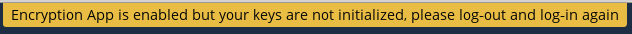
\includegraphics{encryption1.png}
\end{figure}

When you log back in it takes a few minutes to work, depending on how many
files you have, and then you are returned to your default ownCloud page.
\begin{figure}[htbp]
\centering

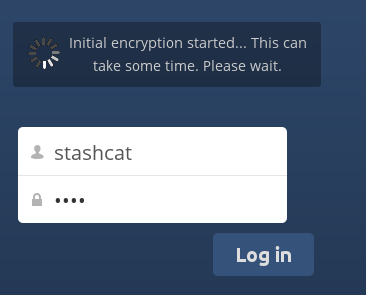
\includegraphics{encryption2.png}
\end{figure}

\begin{notice}{note}{Note:}
You must never lose your ownCloud password, because you will lose
access to your files. Though there is an optional recovery option that your
ownCloud administrator may enable; see the Recovery Key Password section
(below) to learn about this.
\end{notice}


\subsection{Sharing Encrypted Files}
\label{files/encrypting_files:sharing-encrypted-files}
Only users who have private encryption keys have access to shared encrypted
files and folders. Users who have not yet created their private encryption keys
will not have access to encrypted shared files; they will see folders and
filenames, but will not be able to open or download the files. They will see a
yellow warning banner that says ``Encryption App is enabled but your keys are not
initialized, please log-out and log-in again.''

Share owners may need to re-share files after encryption is enabled; users
trying to access the share will see a message advising them to ask the share
owner to re-share the file with them. For individual shares, un-share and
re-share the file. For group shares, share with any individuals who can't access
the share. This updates the encryption, and then the share owner can remove the
individual shares.


\subsubsection{Recovery Key Password}
\label{files/encrypting_files:recovery-key-password}
If your ownCloud administrator has enabled the recovery key feature, you can
choose to use this feature for your account. If you enable ``Password recovery''
the administrator can read your data with a special password. This feature
enables the administrator to recover your files in the event you lose your
ownCloud password. If the recovery key is not enabled, then there is no way to
restore your files if you lose your login password.
\begin{figure}[htbp]
\centering

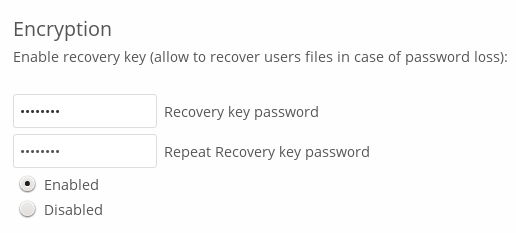
\includegraphics{encryption3.png}
\end{figure}


\subsection{Files Not Encrypted}
\label{files/encrypting_files:files-not-encrypted}
Only the data in your files is encrypted, and not the filenames or folder
structures. These files are never encrypted:
\begin{itemize}
\item {} 
Old files in the trash bin.

\item {} 
Image thumbnails from the Gallery app.

\item {} 
Previews from the Files app.

\item {} 
The search index from the full text search app.

\item {} 
Third-party app data

\end{itemize}

There may be other files that are not encrypted; only files that are exposed to
third-party storage providers are guaranteed to be encrypted.


\subsubsection{Change Private Key Password}
\label{files/encrypting_files:change-private-key-password}
This option is only available if your log-in password, but not your encryption
password, was changed by your administrator. This can occur if your ownCloud
provider uses a external user back-end (for example, LDAP) and changed your
login password using that back-end configuration. In this case, you can set
your encryption password to your new login password by providing your old and
new login password. The Encryption app works only if your login password and
your encryption password are identical.


\section{Using Federation Shares}
\label{files/federated_cloud_sharing:using-federation-shares}\label{files/federated_cloud_sharing::doc}
Federation Sharing allows you to mount file shares from remote ownCloud servers, in effect
creating your own cloud of ownClouds. You can create direct share links with
users on other ownCloud servers.


\subsection{Creating a New Federation Share}
\label{files/federated_cloud_sharing:creating-a-new-federation-share}
Federation sharing is enabled on new or upgraded ownCloud installations
by default. Follow these steps to create a new share with other ownCloud 9 servers:

1. Go to your \code{Files} page and click the Share icon on the file or directory
you want to share. In the sidebar enter the username and URL of the remote user
in this form: \code{\textless{}username\textgreater{}@\textless{}oc-server-url\textgreater{}}. In this example, that is
\code{layla@remote-server/owncloud}. The form automatically echoes the address
that you type and labels it as ``remote''. Click on the label.
\begin{figure}[htbp]
\centering

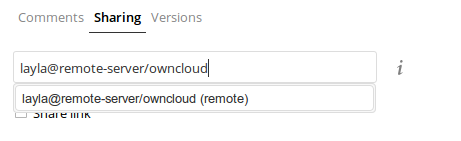
\includegraphics{direct-share-1.png}
\end{figure}

2. When your local ownCloud server makes a successful connection with the remote
ownCloud server you'll see a confirmation. Your only share option is \textbf{Can
edit}.

Click the Share button anytime to see who you have shared your file with. Remove
your linked share anytime by clicking the trash can icon. This only unlinks the
share, and does not delete any files.


\subsection{Creating a New Federated Cloud Share via Email}
\label{files/federated_cloud_sharing:creating-a-new-federated-cloud-share-via-email}
Use this method when you are sharing with users on ownCloud 8.x and older.

What if you do not know the username or URL? Then you can have ownCloud create
the link for you and email it to your recipient.
\begin{figure}[htbp]
\centering

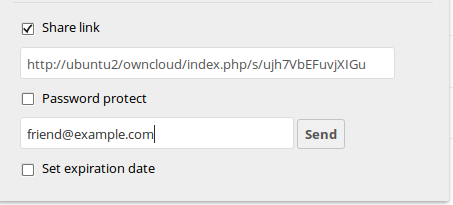
\includegraphics{create_public_share-6.png}
\end{figure}

When your recipient receives your email they will have to take a number of
steps to complete the share link. First they must open the link you sent them in
a Web browser, and then click the \textbf{Add to your ownCloud} button.
\begin{figure}[htbp]
\centering

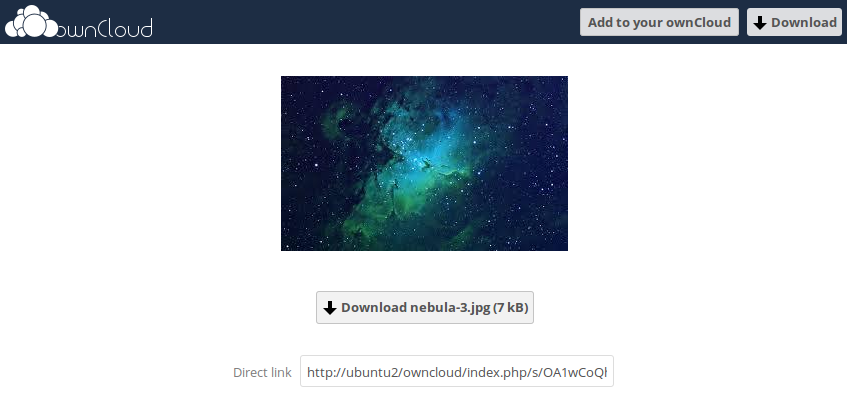
\includegraphics{create_public_share-8.png}
\end{figure}

The \textbf{Add to your ownCloud} button changes to a form field, and your recipient
needs to enter the URL of their ownCloud server in this field and press the
return key, or click the arrow.
\begin{figure}[htbp]
\centering

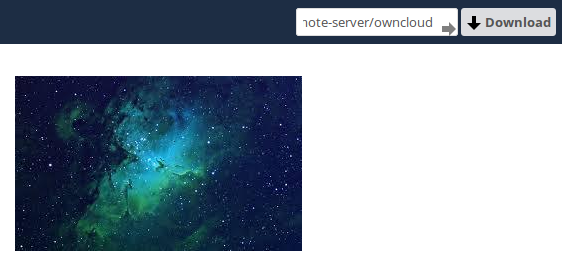
\includegraphics{create_public_share-9.png}
\end{figure}

Next, they will see a dialog asking to confirm. All they have to do is click
the \textbf{Add remote share} button and they're finished.

Remove your linked share anytime by clicking the trash can icon. This only
unlinks the share, and does not delete any files.


\section{Making Anonymous Uploads (Enterprise Only)}
\label{files/file_drop:making-anonymous-uploads-enterprise-only}\label{files/file_drop::doc}
If your ownCloud administrator (Enterprise edition only) has enabled the
Files Drop application, you may create your own special upload directory so that
other people can upload files to you without having to log in to the server, and
without being an ownCloud user. They will not be allowed to see the contents of
this directory, or to make any changes. This is an excellent alternative to
sending large attachments via email, using an FTP server, or using commercial
file-sharing services.


\subsection{Setting Up Your Own File Drop}
\label{files/file_drop:setting-up-your-own-file-drop}
Go to your Personal page and you will see the Files Drop configuration section.

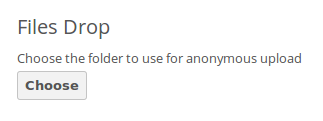
\includegraphics{files-drop-2.png}

Click the \textbf{Choose} button to open a dialog to select your upload directory.
You may wish to first create a special upload directory (on your Files page),
which in the following example is name \textbf{upload}.
\begin{figure}[htbp]
\centering
\capstart

\scalebox{0.500000}{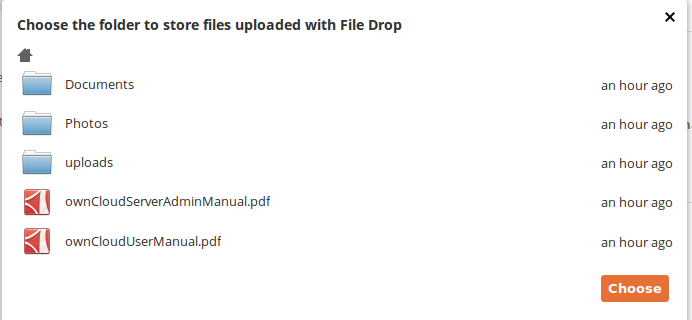
\includegraphics{files-drop-3.png}}
\caption{\emph{Click to enlarge}}\end{figure}

On your Personal page you should now see a URL for your upload directory. Share
this URL with anyone you want to allow uploads to your Files Drop folder. Note
that the default maximum upload size in this example is 512MB; this is
configurable, so contact your ownCloud administrator if you need a larger
limit.

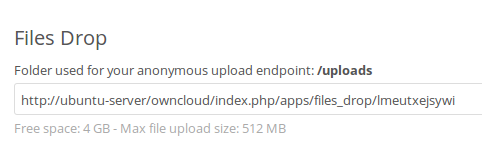
\includegraphics{files-drop-4.png}


\subsection{Uploading Files}
\label{files/file_drop:uploading-files}
Using the Files Drop app is simple. You receive a link to the upload
folder, click the link, and then you'll see an ownCloud page with a \textbf{Click to
upload} button.
\begin{figure}[htbp]
\centering
\capstart

\scalebox{0.500000}{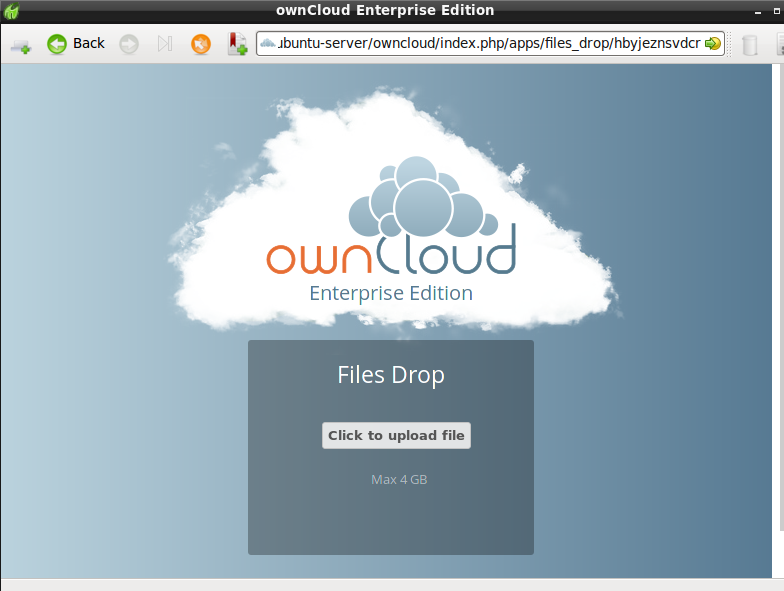
\includegraphics{files-drop-5.png}}
\caption{\emph{Click to enlarge}}\end{figure}

This opens a file picker, and you select the file or directory you want to
upload.
\begin{figure}[htbp]
\centering
\capstart

\scalebox{0.500000}{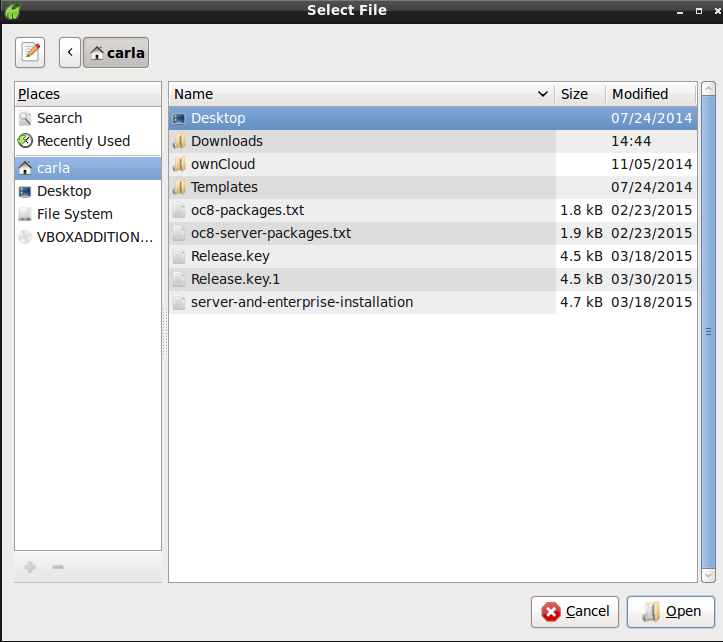
\includegraphics{files-drop-6.png}}
\caption{\emph{Click to enlarge}}\end{figure}

When your upload is completed, you'll see a confirmation message with the
filenames.
\begin{figure}[htbp]
\centering

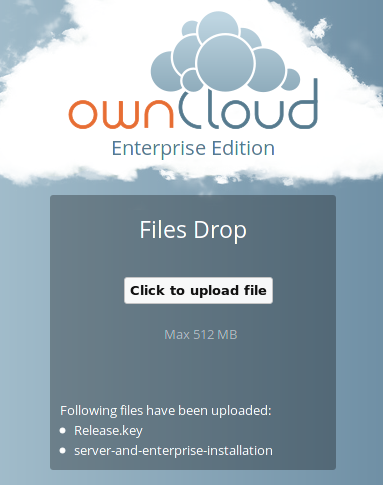
\includegraphics{files-drop-7.png}
\end{figure}


\section{Large File Uploads}
\label{files/large_file_upload:large-file-uploads}\label{files/large_file_upload::doc}
When uploading files through the web client, ownCloud is limited by PHP and
Apache configurations. By default, PHP is configured for only 2 megabyte
uploads. As this default upload limit is not entirely useful, we recommend that
your ownCloud admin increase the ownCloud variables to sizes appropriate for
users.

Modifying certain ownCloud variables requires administrative access.  If you
require larger upload limits than have been provided by the default (or already
set by your administrator):
\begin{itemize}
\item {} 
Contact your administrator to request an increase in these variables

\item {} 
Refer to the section in the \href{https://doc.owncloud.org/server/9.0/admin\_manual/configuration\_files/big\_file\_upload\_configuration.html}{Admin Documentation} that describes how to manage file
upload size limits.

\end{itemize}


\section{Storage Quota}
\label{files/quota:storage-quota}\label{files/quota::doc}
Your ownCloud admin has the option to set a storage quota on users. Look at
the top of your Personal page to see what your quota is, and how much you have
used.
\begin{figure}[htbp]
\centering

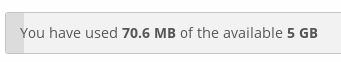
\includegraphics{quota1.png}
\end{figure}

It may be helpful to understand how your quota is calculated.

Metadata (thumbnails, temporary files, cache, and encryption keys) takes up
about 10\% of disk space, but is not counted against user quotas. Some apps
store information in the database, such as the Calendar and Contacts apps. This
data is excluded from your quota.

When other users share files with you, the shared files count against the
original share owner's quota. When you share a folder and allow other users or
groups to upload files to it, all uploaded and edited files count against your
quota. When you re-share files shared with you, the re-share still counts
against the quota of the original share owner.

Encrypted files are a little larger than unencrypted files; the unencrypted size
is calculated against your quota.

Deleted files that are still in the trash bin do not count against quotas. The
trash bin is set at 50\% of quota. Deleted file aging is set at 30 days. When
deleted files exceed 50\% of quota then the oldest files are removed until the
total is below 50\%.

When version control is enabled, the older file versions are not counted against
quotas.

If you create a public share via URL, and allow uploads, any uploaded files
count against your quota.


\section{Version Control}
\label{files/version_control:version-control}\label{files/version_control::doc}
ownCloud supports simple version control system for files. Versioning creates
backups of files which are accessible via the Versions tab on the Details
sidebar. This tab contains the history of the file where you can roll back a
file to any previous version. Changes made at intervals greater than two minutes
are saved in data/{[}user{]}/versions.
\begin{figure}[htbp]
\centering

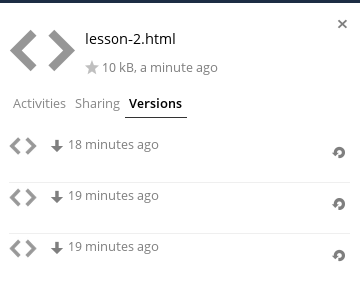
\includegraphics{files_versioning.png}
\end{figure}

To restore a specific version of a file, click the circular arrow to the left.
Click on the timestamp to download it.

The versioning app expires old versions automatically to make sure that
the user doesn't run out of space. This pattern is used to delete
old versions:
\begin{itemize}
\item {} 
For the first second we keep one version

\item {} 
For the first 10 seconds ownCloud keeps one version every 2 seconds

\item {} 
For the first minute ownCloud keeps one version every 10 seconds

\item {} 
For the first hour ownCloud keeps one version every minute

\item {} 
For the first 24 hours ownCloud keeps one version every hour

\item {} 
For the first 30 days ownCloud keeps one version every day

\item {} 
After the first 30 days ownCloud keeps one version every week

\end{itemize}

The versions are adjusted along this pattern every time a new version gets
created.

The version app never uses more that 50\% of the user's currently available free
space. If the stored versions exceed this limit, ownCloud deletes the oldest
versions until it meets the disk space limit again.


\chapter{Contacts \& Calendar}
\label{pim/index:contacts-calendar}\label{pim/index::doc}
The Contacts, Calendar, and Mail apps are not included in ownCloud 9, and are
not supported. You may easily install them by clicking the Enable button on
their respective Apps \textgreater{} Productivity entries.


\section{Using the Contacts App}
\label{pim/contacts:using-the-contacts-app}\label{pim/contacts::doc}
The Contacts app is not enabled by default in ownCloud 9.2 and needs to
be enabled separately. It is also not a supported core app. It is currently
under heavy development, so documentation has moved to the \href{https://github.com/owncloud/documentation/wiki/Using-the-Contacts-App-in-ownCloud-9.0}{documentation Wiki
on Github}.


\section{Using the Calendar App}
\label{pim/calendar::doc}\label{pim/calendar:using-the-calendar-app}
The Calendar app is not enabled by default in ownCloud 9.2 and needs to
be enabled separately. It is also not a supported core app. It is currently
under heavy development, so documentation has moved to the \href{https://github.com/owncloud/documentation/wiki/Using-the-Calendar-App-in-ownCloud-9.0}{documentation Wiki
on Github}. You are welcome to add content to the Wiki document; all you
need is a Github account.


\section{iOS - Synchronize iPhone/iPad}
\label{pim/sync_ios::doc}\label{pim/sync_ios:ios-synchronize-iphone-ipad}

\subsection{Calendar}
\label{pim/sync_ios:calendar}\begin{enumerate}
\item {} 
Open the settings application.

\item {} 
Select Mail, Contacts, Calendars.

\item {} 
Select Add Account.

\item {} 
Select Other as account type.

\item {} 
Select Add CalDAV account.

\item {} 
For server, type \code{example.com/remote.php/dav/principals/users/USERNAME/}

\item {} 
Enter your user name and password.

\item {} 
Select Next.

\item {} 
If your server does not support SSL, a warning will be displayed.
Select Continue.

\item {} 
If the iPhone is unable to verify the account information perform the
following steps:
\begin{itemize}
\item {} 
Select OK.

\item {} 
Select advanced settings.

\item {} 
If your server does not support SSL, make sure Use SSL is set to OFF.

\item {} 
Change port to 80.

\item {} 
Go back to account information and hit Save.

\end{itemize}

\end{enumerate}

Your calendar will now be visible in the Calendar application


\subsection{Address book}
\label{pim/sync_ios:address-book}\begin{enumerate}
\item {} 
Open the settings application.

\item {} 
Select Mail, Contacts, Calendars.

\item {} 
Select Add Account.

\item {} 
Select Other as account type.

\item {} 
Select Add CardDAV account.

\item {} 
For server, type \code{example.com/remote.php/dav/principals/users/USERNAME/}

\item {} 
Enter your user name and password.

\item {} 
Select Next.

\item {} 
If your server does not support SSL, a warning will be displayed.
Select Continue.

\item {} 
If the iPhone is unable to verify the account information perform the
following:
\begin{itemize}
\item {} 
Select OK.

\item {} 
Select advanced settings.

\item {} 
If your server does not support SSL, make sure Use SSL is set to OFF.

\item {} 
Change port to 80.

\item {} 
Go back to account information and hit Save.

\end{itemize}

\end{enumerate}

Now should now find your contacts in the address book of your iPhone.
If it's still not working, have a look at the {\hyperref[pim/troubleshooting::doc]{\emph{Troubleshooting}}}
and \href{https://doc.owncloud.org/server/9.0/admin\_manual/issues/index.html\#troubleshooting-contacts-calendar}{Troubleshooting Contacts \& Calendar} guides.


\section{Synchronizing with OS X}
\label{pim/sync_osx::doc}\label{pim/sync_osx:synchronizing-with-os-x}
To use ownCloud with iCal you will need to use the following URL:

\begin{Verbatim}[commandchars=\\\{\}]
https://example.com/remote.php/dav/principals/users/USERNAME/
\end{Verbatim}

The setup is basically the same as with iOS using the path \code{https://example.com/remote.php/dav/principals/users/USERNAME/}
to sync with ownCloud. For OS X 10.7 Lion and 10.8 Mountain Lion everything works
fine, but OS X 10.6 (Snow Leopard) and older needs some fiddling to work. A user
contributed the following:

\#. Make sure, addressbook is not running. If it is, select the windows and press
Command + Q to terminate it.
\#. Navigate to \textbf{/Users/YOUR\_USERNAME/Library/Application Support/AddressBook/Sources}.
If you already have some kind of addressbook setup, it is likely you will see
some folders named like this \textbf{BEA92826-FBF3-4E53-B5C6-ED7C2B454430}.
Note down what folders there are now and leave the window open.
\#. Open addressbook and try to add a new CardDav addressbook. At this point, it
does not matter what information you enter. It will come up with the same error
message you mentioned before when you click ``Create''. Ignore it and click ``Create''
again. A non-functional addressbook will be added.
\#. Close addressbook again using Command + Q
\#. Go back to the folder window from step 2. You will now see a newly created folder
with another long string as its name.
\#. Navigate to the newly created folder and edit the \textbf{Configuration.plist} with
your favorite text editor.
\#. Search for a section looking like this:

\begin{Verbatim}[commandchars=\\\{\}]
\PYGZlt{}key\PYGZgt{}servername\PYGZlt{}/key\PYGZgt{} \PYGZlt{}string\PYGZgt{}https://:0(null)\PYGZlt{}/string\PYGZgt{} \PYGZlt{}key\PYGZgt{}username\PYGZlt{}/key\PYGZgt{} \PYGZlt{}string\PYGZgt{}Whatever\PYGZus{}you\PYGZus{}entered\PYGZus{}before\PYGZlt{}/string\PYGZgt{}
\end{Verbatim}
\begin{enumerate}
\setcounter{enumi}{7}
\item {} 
Make it look like this. Please note that the :443 after \textbf{example.com} is important:

\begin{Verbatim}[commandchars=\\\{\}]
\PYGZlt{}key\PYGZgt{}servername\PYGZlt{}/key \PYGZlt{}string\PYGZgt{}https://example.com:443/owncloud/remote.php/dav/principals/users/USERNAME\PYGZlt{}/string\PYGZgt{} \PYGZlt{}key\PYGZgt{}username\PYGZlt{}/key \PYGZlt{}string\PYGZgt{}username\PYGZlt{}/string\PYGZgt{}
\end{Verbatim}

\item {} 
Save the file and open addressbook again. It will not work yet.

\item {} 
Open the preferences for your ownCloud CardDAV-Account and enter your password.

\item {} 
You may have to restart addressbook once more. After this, it should work.

\end{enumerate}

If it's still not working, have a look at the {\hyperref[pim/troubleshooting::doc]{\emph{Troubleshooting}}} and
\href{https://doc.owncloud.org/server/9.0/admin\_manual/issues/index.html\#troubleshooting-contacts-calendar}{Troubleshooting Contacts \& Calendar} guides.

There is also an easy \href{https://forum.owncloud.org/viewtopic.php?f=3\&t=132}{HOWTO} in the forum.


\section{Synchronizing with KDE SC}
\label{pim/sync_kde:synchronizing-with-kde-sc}\label{pim/sync_kde::doc}
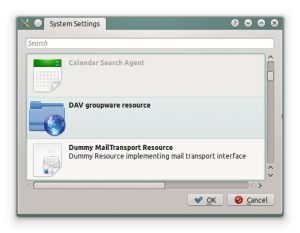
\includegraphics{kdes1.png}

From KDE SC 4.8 and forward setting up ownCloud is very easy. Note that the KDE
calendar needs to have the ownCloud Calendar and Contacts apps enabled on the
ownCloud server. You need both and not just the Calendar. From System Settings
Personal Information/Akonadi Resources Configuration select DAV Groupware
resource.

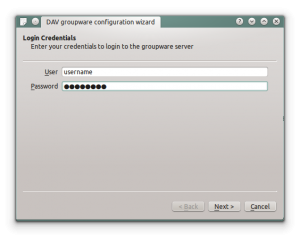
\includegraphics{kdes2.png}

Enter your ownCloud username and password and click ``Next''.

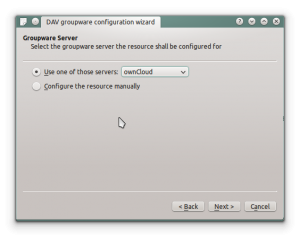
\includegraphics{kdes3.png}

Select ownCloud in the drop down list and click ``Next''.

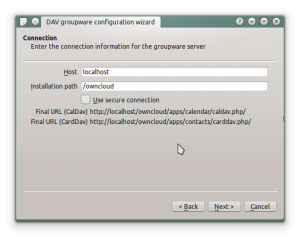
\includegraphics{kdes4.png}

Enter the host name and installation path. If you do not use SSL
remember to de-select ``Use secure connection''.

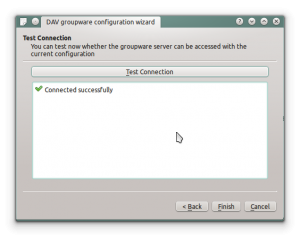
\includegraphics{kdes5.png}

Test the connection. If everything went well you should see a message
like the one below.

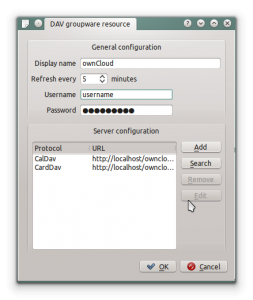
\includegraphics{kdes6.png}

Click ``Finish'' and you will be able to change the display name and
refresh interval.

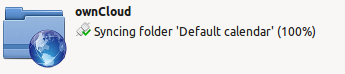
\includegraphics{kdes7.png}

Now you should see the Akonadi resource doing the first
synchronization.

You can find the Contacts and Calendars in Kontact (or
KOrganizer/KAddressbook if you run the programs separately.)

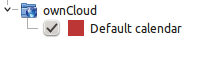
\includegraphics{kdes9.png}

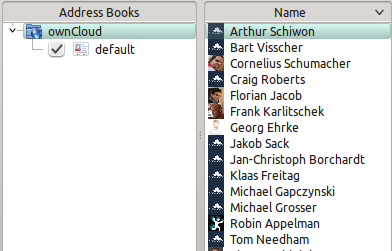
\includegraphics{kdes.png}


\section{Thunderbird - Synchronize Addressbook}
\label{pim/sync_thunderbird::doc}\label{pim/sync_thunderbird:thunderbird-synchronize-addressbook}

\subsection{Addressbook}
\label{pim/sync_thunderbird:addressbook}
As someone who is new to ownCloud, New to SoGo Connector, and new to Thunderbird Addressbook... here is what you need in excruciating pithy detail to make this work (for all the other lost souls out there):
\begin{enumerate}
\item {} 
\href{http://www.mozilla.org/en-US/thunderbird/}{Thunderbird} for your OS unless it comes with your OS distribution (Linux)

\item {} 
\href{http://www.sogo.nu/downloads/frontends.html}{Sogo Connector} (latest release)

\item {} 
\href{https://addons.mozilla.org/en-US/thunderbird/addon/lightning/}{Lightning} (a Thunderbird calendar add-on. At the time (Aug 14), syncing your contacts only works with this add-on installed.)

\end{enumerate}

With an installed Thunderbird mailtool, an installed SoGo Connector, and an installed Lightning add-on:
\begin{enumerate}
\item {} 
Thunderbird Addressbook is in the Thunderbird ``Tools'' Menu

\item {} 
In the Thunderbird Addressbook application:
\begin{itemize}
\item {} 
``File \textgreater{} New \textgreater{} \textbf{Remote Addressbook}'' (SoGo Connector added this)

\item {} 
``\textbf{Name:}'' is the name you want to give your Addressbook in the Thunderbird addressbook bar area

\item {} 
``\textbf{URL:}'' is found in your ownCloud Contacts area, that little Gear symbol

\end{itemize}

\end{enumerate}

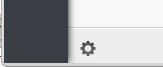
\includegraphics{contact_thunderbird-Symbol_Gear.jpg}

in the -bottom left- of the Contacts View (same symbol as found in the -top right- in the Calendar view). Then look for a little impeller symbol

\includegraphics{contact_thunderbird-Symbol_Impeller.jpg}

which will display the URL you need for your installation to work.

\includegraphics{contact_thunderbird-URL_config.jpg}

Once installed, synchronize (right click on your newly made remote address book and select ``Synchronize'').
You'll see your address book populate from ownCloud! Don't click ``read only'' above unless you don't want to
modify your ownCloud server addressbook, like it contains a listing of corporate contacts and is shared with
lots of people, and you don't want a new user dragging it somewhere unintended.

The rest of the details of dealing with Thunderbird addressbook are left to the reader... First thing I learned
is dragging a contact to a different addressbook is a ``move'' operation. If you are worried about losing the
contact, save it to a VCF file using ownCloud (Or LDIF using Thunderbird Addressbook) first! Like dragging
from ``ownCloud Addressbook'' to ``Personal Address Book'' removes the contact from ownCloud Server
(\emph{deleting it from all the other synchronized installations}) and puts it in your Local Machine -only-
Address Book. So be careful or you'll have unintended consequences where you might have intended a ``copy'' operation.

Contact \emph{Pictures} are also sync'ed!


\section{Troubleshooting}
\label{pim/troubleshooting::doc}\label{pim/troubleshooting:troubleshooting}

\subsection{BlackBerry OS 10.2}
\label{pim/troubleshooting:blackberry-os-10-2}
BlackBerry OS up to 10.2.2102 does not accept a URL with protocol \code{https://}
in front of the server address. It will always tell you that it cannot login on
your server. So instead of writing:

\begin{Verbatim}[commandchars=\\\{\}]
https://example.com/remote.php/dav/principals/users/USERNAME/
\end{Verbatim}

in the server address field, you have to write:

\begin{Verbatim}[commandchars=\\\{\}]
example.com/remote.php/dav/principals/users/USERNAME/
\end{Verbatim}


\chapter{Collaborative Document Editing}
\label{documents:collaborative-document-editing}\label{documents::doc}
The Documents application supports editing documents within ownCloud, without
the need to launch an external application. The Documents app supports these
features:
\begin{itemize}
\item {} 
Cooperative edit, with multiple users editing files simultaneously.

\item {} 
Document creation within ownCloud.

\item {} 
Document upload.

\item {} 
Share and edit files in the browser, and then share them inside ownCloud or
through a public link.

\end{itemize}

Supported file formats are \emph{.odt}, \emph{.doc}, and \emph{.docx}.


\section{The main interface}
\label{documents:the-main-interface}
\includegraphics{oc_documents.png}


\subsection{Create or Upload a Document}
\label{documents:create-or-upload-a-document}
In the Documents application, you can upload an existing document or create a
new one. The \emph{New document} button creates a document named ``New
document.odt''. The extension ODT is an OpenDocument format, which is supported
by most word processors including Microsoft Word, LibreOffice Writer, and
OpenOffice Writer.


\subsection{Edit a Document}
\label{documents:edit-a-document}
To edit a document, access the Documents app from your Apps menu at the top
left of your ownCloud window.

\includegraphics{oc_documents_edit.png}
\begin{enumerate}
\item {} 
Click on the file name to change it.

\item {} 
Share your document (See the {\hyperref[documents:share-a-document]{\emph{Share a document}}} section.)

\item {} 
Formatting toolbar.

\item {} 
Zoom in/out

\item {} 
Close and save.

\item {} 
Users currently editing this document.

\end{enumerate}


\subsubsection{Collaboratively Editing a Document}
\label{documents:collaboratively-editing-a-document}
To edit a file collaboratively, it must be shared with everyone who needs
editing permissions. Multiple users can edit it at the same time, and changes
appear as they are made. The cursor of each user is the same color as the
border color of their user picture.

If a user is not a local user (e.g accessing the file using public link), they
will be shown as guest in the user list, automatically named Guest 1, Guest 2,
and so on. Guests can change their nicknames at any time by clicking on their
names or thumbnails in the user list.


\subsection{Delete a Document}
\label{documents:delete-a-document}
You can't delete a document from inside the Document app, but must go to your
Files page and delete it from there. You'll find it in your default documents
directory, which is configured on your ownCloud Personal page (see
{\hyperref[userpreferences::doc]{\emph{Setting Your Preferences}}}.)


\subsection{Share a Document}
\label{documents:id1}\label{documents:share-a-document}
Document sharing has the same options as when sharing other files. While editing
a document, you can use the \emph{Share} button to enable other users to edit the
document. This button will display all available options to share.


\chapter{Setting Your Preferences}
\label{userpreferences:setting-your-preferences}\label{userpreferences::doc}
As a user, you can manage your personal settings.

To access your personal settings:
\begin{enumerate}
\item {} 
Clicking on your username in the top, right corner of your ownCloud instance.

The Personal Settings Menu opens.
\begin{figure}[htbp]
\centering

\includegraphics{oc_personal_settings_dropdown.png}
\end{figure}

\emph{Personal Settings Menu}

\item {} 
Choose \emph{Personal} from the drop down menu.
\begin{figure}[htbp]
\centering

\includegraphics{personal_settings.png}
\end{figure}

\end{enumerate}

\begin{notice}{note}{Note:}
If you are an administrator, you can also manage users and administer
the server. These links do not appear to a non-admin user.
\end{notice}

The options listed in the Personal Settings Page depend on the applications that
are enabled by the administrator.  Some of the features you will see
include the following.
\begin{itemize}
\item {} 
Usage and available quota

\item {} 
Manage your profile picture.

\item {} 
Full name. You can make this anything you want, as it is separate from your
ownCloud login name, which is unique and cannot be changed.

\item {} 
Email address.

\item {} 
Lists your Group memberships.

\item {} 
Manage your password.

\item {} 
{\hyperref[userpreferences::doc]{\emph{Setting Your Preferences}}}.

\item {} 
Choose the language for your ownCloud interface.

\item {} 
Links to desktop and mobile apps.

\item {} 
Manage your Activity stream and notifications.

\item {} 
Default folder to save new documents to.

\item {} 
Your Federated sharing ID.

\item {} 
Social sharing links.

\item {} 
ownCloud version.

\end{itemize}


\chapter{Manage Connected Browsers and Devices}
\label{session_management:manage-connected-browsers-and-devices}\label{session_management::doc}
The personal settings page allows you to have an overview on the connected
browsers and devices.


\section{Managing Connected Browsers}
\label{session_management:managing-connected-browsers}
In the list of connected browsers you see which browsers connected to your
account recently:
\begin{quote}
\begin{figure}[htbp]
\centering

\includegraphics{settings_sessions.png}
\end{figure}
\end{quote}

You can use the trash icon to disconnect any of the browsers in the list.


\section{Managing Devices}
\label{session_management:managing-devices}
In the list of connected devices you see all the devices and clients you
generated a device password for and their last activity:
\begin{quote}
\begin{figure}[htbp]
\centering

\includegraphics{settings_devices.png}
\end{figure}
\end{quote}

You can use the trash icon to disconnect any of the devices in the list.

At the bottom of the list you find a button to create a new device-specific
password. You can choose a name to identify the token later. The generated
password is used for configuring the new client. Ideally, generate individual
tokens for every device you connect to your account, so you can disconnect
those individually if necessary.
\begin{quote}
\begin{figure}[htbp]
\centering

\includegraphics{settings_devices_add.png}
\end{figure}
\end{quote}

\begin{notice}{note}{Note:}
You have only access to the device password when creating it,
ownCloud will not save the plain password, hence it's recommended to
enter the password on the new client immediately.
\end{notice}

\begin{notice}{note}{Note:}
If two-factor authentication is enabled for your account,
device-specific passwords are the only way to configure clients. The
client will deny connections of clients using your login password then.
\end{notice}


\chapter{External Storage}
\label{external_storage/index:external-storage}\label{external_storage/index::doc}

\section{Configuring External Storage}
\label{external_storage/external_storage::doc}\label{external_storage/external_storage:configuring-external-storage}
The External Storage application allows you to mount external storage services,
such as Google Drive, Dropbox, Amazon S3, SMB/CIFS fileservers, and FTP servers
in ownCloud. Your ownCloud server administrator controls which of these are
available to you. Please see \href{https://doc.owncloud.org/server/9.0/admin\_manual/configuration\_files/external\_storage\_configuration\_gui.html}{Configuring External Storage (GUI)} in the ownCloud Administrator's
manual for configuration howtos and examples.


\section{Connecting to SharePoint (Enterprise only)}
\label{external_storage/sharepoint_connecting:connecting-to-sharepoint-enterprise-only}\label{external_storage/sharepoint_connecting::doc}
Native SharePoint support has been added to ownCloud Enterprise Subscription as
a secondary storage location for SharePoint 2007, 2010 and 2013. To the user,
these appear as normal ownCloud mounts, with bi-directional updates in any
ownCloud client: desktop, mobile, or Web. There is one difference, and that is
ownCloud sharing is intentionally disabled for SharePoint mountpoints in order
to preserve SharePoint access controls, and to ensure that content is properly
accessed as per SharePoint rules.

Your ownCloud admin may optionally allow users to mount their own SharePoint
libraries.


\subsection{Accessing SharePoint Folders}
\label{external_storage/sharepoint_connecting:accessing-sharepoint-folders}
When you first log in to ownCloud, the Web interface shows a gray bar behind all
SharePoint folders. The gray bar disappears when the mountpoint is verified by
the server. If you see a red error bar, you'll see either an hourglass that
indicates a connection error, or a key to indicate that authentication is
required.

Your ownCloud admin has the option to configure SharePoint credentials so that
you are authenticated automatically, or you may be required to enter your
credentials. If you have to enter your credentials, click the red bar and you'll
get a login window. You should only have to do this once, as ownCloud will store
your credentials.

If your SharePoint login ever changes, go to your Personal page to update it in
the \code{Sharepoint Personal Configuration} section.


\subsection{Personal Page}
\label{external_storage/sharepoint_connecting:personal-page}
You can manage your SharePoint connections in the \code{Sharepoint Personal
Configuration} section of your ownCloud Personal page. You'll see two sections:
the \code{Admin added mount points} section lists SharePoint mounts controlled by
your ownCloud admin. If users have permissions to mount their own SharePoint
libraries you'll also see a \code{Personal mount points} section.

There are two types of authentication available to you. If you have multiple
SharePoint libraries that use the same authentication, enter your credentials
in \code{Sharepoint Personal Configuration}. Then follow these steps to add your
libraries:
\begin{itemize}
\item {} 
Enter the name of your local mountpoint in the \code{Local Folder Name} column.
This can be an existing folder, or automatically create a new one.

\item {} 
Enter your SharePoint server URL.

\item {} 
Click the little refresh icon to the left of the \code{Document Library} field.
If your credentials and URL are correct you'll get a dropdown list of SharePoint
libraries to choose from.

\item {} 
Select the document library you want to mount.

\item {} 
Select ``Use user credentials''.

\item {} 
Click the \code{Save} button, and you're done

\end{itemize}

You may elect to use different authentication credentials for some of your
SharePoint libraries. For these, you must first select \code{use custom
credentials}, and then fill in the mountpoint and SharePoint site URL. Then
ownCloud can authenticate you, and you can click the refresh icon to see your
libraries. Then select the library you want to mount and click the \code{Save}
button.


\chapter{Using the Bookmarks App}
\label{bookmarks:using-the-bookmarks-app}\label{bookmarks::doc}
The Bookmark application allows you to bookmark Web sites inside ownCloud.


\section{The main interface}
\label{bookmarks:the-main-interface}

\subsection{Add a bookmark}
\label{bookmarks:add-a-bookmark}
In the Bookmark application, enter a URL into the top-left area of the content section. After adding an address, click on the pencil button to edit fields for the given address.
The main ownCloud bookmark interface contains 3 fields at the top where
you can enter the website address (or URL), the title of your bookmark, and
a set of tags separated from each other by a space.
\begin{figure}[htbp]
\centering
\capstart

\includegraphics{bookmark_addurl.png}
\caption{Adding a bookmark manually}\end{figure}

In this example, we have added the page \emph{http://wikipedia.org} with the title ``Wikipedia''
and some tags describing what Wikipedia is for an easier search later on.


\subsection{Edit/Delete a bookmark}
\label{bookmarks:edit-delete-a-bookmark}
You also have the possibility to edit or delete a bookmark.

To edit a bookmark, hover over the bookmark and click on the pencil icon.
The bookmark details will then be filled into the 3 fields at the top of the screen.
Modify your bookmark to your needs then click the save button to persist the change.

To delete a bookmark, hover over the bookmark and click the cross icon.


\subsection{Search}
\label{bookmarks:search}
If you click on a tag, ownCloud will only display the bookmarks that
are described with this tag.

You can also use the search bar of ownCloud in the top right of your screen.

Simply click on the ``Bookmarks'' menu in the sidebar to come back to
the default view.


\section{The Bookmarklet}
\label{bookmarks:the-bookmarklet}\begin{figure}[htbp]
\centering
\capstart

\includegraphics{bookmark_setting.png}
\caption{Bookmarklet link}\end{figure}

The creator of this app understands that people won't want to
open the ownCloud boorkmarks page to add a bookmark every time they see a cool site.
This is why they have made this cool ``bookmarklet''.

A bookmarklet is small button that you can drag and drop in your bookmarks.
The next time you see a cool new site, click on this special bookmark
to add the site to your ownCloud bookmarks.

To find this bookmark, click on the gear button at the bottom of the bookmarks app.



\renewcommand{\indexname}{Index}
\printindex
\end{document}
